\documentclass[extra,referee]{gji}

\usepackage{graphicx}
\usepackage{amsmath}
\usepackage{amsfonts}


% --- Defining math operators ---
\newcommand{\curl}[1]{\ensuremath{\nabla\times \mathbf{#1}}}
\newcommand{\curlSym}[1]{\ensuremath{\nabla\times \boldsymbol{#1}}}
\renewcommand{\div}{\nabla\cdot\,}
\newcommand{\mb}[1]{\ensuremath { {\mathbf #1}}}
\newcommand{\mbSym}[1]{\ensuremath{\boldsymbol{#1}}}
\renewcommand{\deg}{\ensuremath{^\circ}}
\pdfoptionpdfminorversion=6

\graphicspath{{Figures/}}


\begin{document}

\title{Inversion using spatially variable mixed $\ell_p$-norms}

%\renewcommand{\thefootnote}{\fnsymbol{footnote}}

\author{Dominique Fournier\footnotemark[1] and Douglas W. Oldenburg\footnotemark[1]}
\author[D. Fournier, D. W. Oldenburg]
% {Dominique Fournier$^1$ and Douglas W. Oldenburg$^1$ \\
% $^1$ Geophysical Inversion Facility, Department of Earth, Ocean, and Atmospheric Sciences,\\
% University of British Columbia, Canada
% }

\maketitle

\begin{abstract}

Non-uniqueness in the geophysical inverse problem is well recognized and so too is the ability to obtain solutions with different character by altering the form of the regularization function. Of particular note is the use of $\ell_p$-norms with $p \in [0,2]$ which gives rise to sparse or smooth models. Most algorithms are designed to implement a single $\ell_p$-norm for the entire model domain. This is not adequate when the fundamental character of the model changes throughout the volume of interest. In such cases we require a generalized regularization function where each sub-volume of the model domain has penalties on smallness and roughness and its own suite of $\ell_p$ parameters.

Solving the inverse problem using mixed $\ell_p$-norms in the regularization (especially for $p<1$) is computationally challenging. We use the Lawson formulation for the $\ell_p$-norm and solve the optimization problem with Iterative Reweighted Least Squares. The algorithm has two stages; we first solve the $l_2$-norm problem and then we switch to the desired suite of $\ell_p$-norms; there is one value of $p$ for each term in the objective function. To handle the large changes in numerical values of the regularization function when $p$-values are changed, and to ensure that each component of the regularization is contributing to the final solution, we successively rescale the gradients in our Gauss-Newton solution. An indicator function allows us to evaluate our success in finding a solution in which components of the objective function have been equally influential.

We use our algorithm to generate an ensemble of solutions with mixed $\ell_p$-norms. This illuminates some of the non-uniqueness in the inverse problem and helps prevent over-interpretation that can occur by having only one solution. In addition, we use this ensemble to estimate the suite of ${p}$-values that can be used in a final inversion. First, the most common features of our ensemble are extracted using principal component analysis and edge detection procedures; this provides a reference model. A correlation of each member of the ensemble with the reference model, carried out in a windowed domain, then yields a set of ${p}$-values for each model cell. The efficacy of our technique is illustrated on a synthetic 2D cross-well example. We then apply our technique to the field example that motivated this research, the 3D inversion of magnetic data at a kimberlite site in Canada. Since the final regularization terms have different sets of $p$-values in different regions of model space we are able to recover compact regions associated with the kimberlite intrusions, continuous linear features with sharp edges that are associated with dykes, and a background that is relatively smooth. The result has a geologic character that would not have been achievable without the use of spatially variable mixed norms.

\end{abstract}

\begin{keywords}
Numerical modeling, Inverse theory, Magnetic anomalies: modeling and interpretation, North America, Tomography
\end{keywords}

\section{Introduction}
In the general inverse problem we are given data $\mathbf{d^{obs}} = \{d_i^{obs}\}$ some estimate of their uncertainties $\{\sigma_i\}$ and an ability to carry out forward simulations $F_i[m]=d_i^{pred}$. We search for the model $m$ that gave rise to the data. A key issue related to the inverse problem is that there are an infinite number of possible models that can satisfy the observed data, that is, the inverse problem is ill-posed. Various assumptions must be made to reduce the solution to a few plausible candidates. A widespread and successful approach is to pose the inversion as an optimization problem

\begin{equation}
\begin{split}\label{GenMinProb}
\underset{\mathbf{m}}{\text{min}}\; \phi(m) & = \; \phi_d + \beta \phi_m \\
\text{s.t.} \; \phi_d & \leq \phi_d^* \; .
\end{split}
\end{equation}
In \eqref{GenMinProb}, $\phi_d$ is the misfit function
\begin{equation}\label{eq:misfit}
\phi_d =\sum_{i=1}^{N}\left(\frac{d_i^{pred} - {d}_i^{obs}}{\sigma_i}\right)^2 \;,
\end{equation}
and $\phi_m$ is the regularization, or model objective function. It plays a central role in determining the character of the final model. It can take many forms but a generic representation, when we attempt to find 3D functions that characterize an earth volume, is
\begin{equation}
\begin{split}\label{intSmall}
\phi_m &= \sum_{j=s,x,y,z} \alpha_j \int_V |f_j (m)|^{p_j} \;dV\;. \\
\end{split}
\end{equation}
The functions $f_j$ are user-defined but most often have the following form
\begin{equation}
\begin{split}\label{fj}
f_s= m,\;f_x= \frac{d m}{dx},\; f_y= \frac{d m}{dy},\;f_z= \frac{d m}{dz}\;.
\end{split}
\end{equation}
Thus $f_s(m)$ measures the size of $m$ and $f_x(m)$, $f_y(m)$ and $f_z(m)$ measure the roughness along orthogonal directions in 3D. These functionals can also include a reference model $m^{ref}$. For ease of notation we shall omit explicit reference to $m^{ref}$; this is equivalent to setting $m^{ref}=0$. The parameters $p_j$ specify the values of the $\ell_p$ norm (generally $0 \leq p \leq 2$) that can be applied to each of the terms; their choice controls the character of the final model. Solutions with progressively fewer non-zero values of $f_j$ are obtained by successively reducing $p$ from $p=2 \rightarrow 0$. The other important elements in the regularization are the $\alpha$'s; they are user-defined scalars that adjust the relative influence of the various terms in the regularization function.
Finally $\beta$ is a scalar trade-off parameter (often called the Tikhonov parameter) that adjusts the relative weighting of $\phi_m$ and $\phi_d$ in the optimization problem. It is usually chosen so that the final misfit reaches a target value $\phi_d^*$ or is acceptably small.


The optimization problem is often solved by discretizing the system, linearizing the equations about a current model and using a gradient descent algorithm, such as a Gauss-Newton approach, where we attempt to find a solution that has zero gradients
\begin{equation}\label{gradPhi}
\mathbf{g} = \frac{\partial \phi(\mathbf{m})}{\partial \mathbf{m}} = \frac{\partial \phi_d}{\partial \mathbf{m}} + \beta \left[ \alpha_s \frac{\partial \phi_s}{\partial \mathbf{m}} + \alpha_x \frac{\partial \phi_x}{\partial \mathbf{m}} + \alpha_y \frac{\partial \phi_y}{\partial \mathbf{m}} + \alpha_z \frac{\partial \phi_z}{\partial \mathbf{m}} \right] = \mathbf{0} \;.
\end{equation}
where $\mathbf{m}$ refers to a discrete model based on the choice of parameterization.
A solution to \eqref{gradPhi} can readily be calculated by gradient descent methods \cite[]{HestenesStiefel1952, NocedalWright99}.
Most often $\ell_2$-norms are used and this leads to a quadratic regularization function. For instance, the discretized form of \eqref{intSmall} is
\begin{equation}\label{leastSquaresLin}
\begin{split}
\phi_m &= \alpha_s \|\mathbf{V}_s \;\mathbf{m}\|_2^2 + \sum_{j=x,y,z} \alpha_j \|\mathbf{V}_j \;\mathbf{G}_j \;\mathbf{m}\|_2^2 \;,\\
\end{split}
\end{equation}
such that $\mathbf{V}_s,\;\mathbf{V}_x,\;\mathbf{V}_y,$ and $\mathbf{V}_z$ are diagonal matrices relating to the “volumes” of the cells used in discretizing the problem, and
$\mathbf{G}_x,\;\mathbf{G}_y,$ and $\mathbf{G}_z$ are discrete gradient operators. What is sometimes sought, at least as a first pass, is that if $\alpha_s \phi_s$ and $\alpha_x \phi_x$ have about the same numerical value then the two penalty terms are contributing equally. Dimensional analysis shows that for a uniform discretization $h$:
\begin{equation}\label{lengthScale}
\frac{[\phi_x] }{ [\phi_s]} = {[h]}^{-p}\;,
\end{equation}
Thus for the $\ell_2$-norm regularization $\alpha_s/\alpha_x = h^{-2}$.
If the forward problem is linear then the inverse problem (for a fixed $\beta$) is a linear system and easily solved.

Although convenient, the $\ell_2$-norm can be restrictive from the viewpoint of exploring model space. This has prompted the use of other $\ell_p$-norms. The $\ell_1$-norm has received considerable attention. When applied to the smallness term it yields `spikey` or impulsive models; when applied to the derivative term, it yields layered or blocky solutions \cite[]{Li93, FarquharsonOldenburg98, Daubechies10}. The benefits of $\ell_0$-norm have also been realized in generating minimum support models. When applied to the smallness component it gives a sparse model, when applied to the derivative term it gives compact objects \cite[]{Portniaguine1999, LastKubik83,BarbosaSilva94, Ajo-Franklin07}. Other solutions on the full range for $0\leq p\leq 2$ can help widen the search, but $\ell_0$, $\ell_1$, and $\ell_2$ often form the main applications.


In most applications the same norm has been applied uniformly to all components $f_j(m)$ making up the regularization, either globally or locally \cite[]{SunLi14}. A next step, which we are taking in this paper, is to use different norms for different components of \eqref{intSmall}. The motivation is that the character of the model might change throughout the volume of interest; for instance it could be smooth and sparse in one region, and small and blocky in another. As an example, consider the magnetic data shown in (Figure~\ref{TKC_Data}). This is a total field magnetic map taken over the Tli Kwi Cho (TKC) kimberlite deposit, Northwest Territories. Different geologic structural features are evident: (a) linear structures corresponding to dykes, (b) compact bodies corresponding to kimberlite pipes, (c) a background host unit that is smoothly varying. An inversion algorithm that uses different $\ell_p$-norms in different regions could capture the essence of this geology.
\begin{figure}
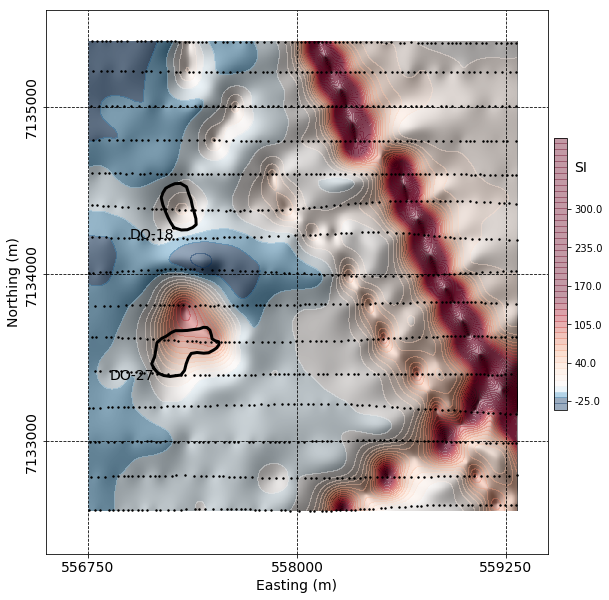
\includegraphics[width=\columnwidth]{Figures/MAG_TKC_DataMap.png}
\caption{TMI data map from an airborne DIGHEM survey flown in 1992 over the DO-18/27 kimberlite pipes, formerly known as the Tli Kwi Cho (TKC) deposit, Northwest Territories. The study area comprises both linear and compact features of interest.}
\label{TKC_Data}
\end{figure}

Our paper has two parts. In the first, we develop a stable two-stage algorithm for carrying out the optimization of spatially variable mixed norm (SVMN) objective functions. The essential part of this algorithm is to introduce an iterative re-scaling of the partial derivatives so that different components of the objective function can impact the solution throughout the inversion process. To illustrate our procedure we use the 2D seismic tomography problem of \citet{SunLi14}. We define an indicator function that allows us to evaluate our success in finding a solution in which components of the objective function have been equally influential. To implement the general $l_p$-norm measure we use the Lawson approximation \cite[]{Lawson61}.

The development of a stable algorithm for solving multi-component objective functions with variable $\ell_p$-norm allows us to generate solutions that have different character and, partially, explore solution space. Our approach is to carry out a set of inversions that use different combinations of $\ell_p$-norms. The suite of models generated can be subjected to further analysis. We use Principal Component Analysis (PCA) and edge detection algorithms to define dominant features and then use those images to determine $\ell_p$-norms relevant to any particular sub-domain of the model. The efficacy of our approach is shown by carrying out SVMN inversions of the magnetic data shown in Figure~\ref{TKC_Data}.


\section{Methodology}

In this study we focus on the general $\ell_p$-norm measures of the form:
\begin{equation} \label{eq:lpreg}
\phi_s^{p} = \sum_{i} {|m_i|}^{p} \;,
\end{equation}
to constrain the inverse problem in \eqref{GenMinProb}.
Several approximations to the $\ell_p$-norm have been implemented so that the function remains differentiable at $m_i = 0$. Approximations such as the Huber norm \cite[]{Huber64}
\[
\sum_{i} {|m_i|}^p \approx \sum_{i} \left\{\begin{array}{lr}
m_i^2, & |m_i| \leq \epsilon,\\
2\epsilon|m_i|-\epsilon^2, & |m_i| > \epsilon,
\end{array}\right\}
\]
and the Ekblom norm \cite[]{Ekblom73}:
\begin{equation}\label{Ekblom}
\sum_{i} {|m_i |}^p \approx \sum_{i} {(m_i^2 + \epsilon^2)}^{p/2} \;
\end{equation}
have been used to approximate the $\ell_1$-norm, where a small threshold value $\epsilon$ is added \cite[]{Li93, Gorodnitsky97, FarquharsonOldenburg98}.
Similarly, the $\ell_p$-norm can be approximated by Lawson's algorithm \cite[]{Lawson61}:
\begin{equation} \label{eq:Lawson}
\sum_{i} {|m_i |}^p \approx \sum_{i}\frac{m_i^2}{{{(m_i^{2} + \epsilon^2 )}^{1-p/2}} }
\end{equation}
This formulation has received considerable attention in the literature and emerged as an important method in geophysical inversion.
%Figure~\ref{NormIRLS} compares the $\ell_p$-norms with the Lawson approximation over a range of model values. As $\epsilon \rightarrow 0$, the approximation approaches the $\ell_p$-norm on the complete interval $p \in [0, 2]$.
%\begin{figure}
%\includegraphics[width=\columnwidth]{Figures/NormIRLS.png}
%\caption{Approximated $\ell_p$-norm using the Lawson measure \cite[]{Lawson61} over a range of $p$-values and for a fixed threshold parameter $\epsilon=10^{-1}$.}
%\label{NormIRLS}
%\end{figure}
Under this approximation, the $\ell_p$-norm penalty \eqref{intSmall} takes the form:
\begin{equation}\label{eq:IntegralIRLS}
\begin{split}
	\int_V | f(m) |^{p_j} \;dV \approx \int_V{\frac{ {f (m)}^2}{\left( {{f (m)}}^{2} + \epsilon_j^2 \right)^{1-p_j/2 }}\;dV} \;,
\end{split}
\end{equation}
where once again $f(m)$ from \eqref{fj} can either be a measure of the model or its spatial gradients, and $m$ may, or may not be replaced by $m-m^{ref}$.
The function can be discretized and evaluated through the Iterative Reweighted Least-Squares (IRLS) approach where the denominator is replaced by model parameters from the most recent iteration. The smallest model component can be written as:
\begin{equation} \label{eq:IRLS}
\phi_s^{p_s} = \sum_{i}\frac{m_i^2}{{{((m^{(k-1)}_i)^{2} + \epsilon_s^2 )}^{1-p_s/2}} }V_i
\end{equation}
where $m_i^{(k-1)}$ are model parameters obtained at a previous iteration and $V_i$ are “volume” terms connected with the discretization. In \eqref{eq:IRLS} we have explicitly written the objective function as $\phi_s^{p_s}$ to indicate that we are evaluating a smallest model component with an $\ell_p$-norm with
$p=p_s$.
The approximated norm can be expressed in linear form as:
\begin{equation}\label{IRLSphis}
\phi_s^{p_s} = \| \mathbf{V}_s\:\mathbf{R}_s\:\mathbf{m}\|_2^2 \;,
\end{equation}
\begin{equation}\label{eq:R_w}
\begin{split}
	\mathbf{R}_s &= \text{diag} \left[{\Big( {({\mathbf{m}}^{(k-1)})}^{2} + \epsilon_s^2 \Big)}^{p_s/2 - 1} \right]^{1/2} \;.
\end{split}
\end{equation}
Carrying out the same IRLS operation on the derivative components yields
\begin{equation}\label{phixMatrix}
\phi_j^{p_j} = \| \mathbf{V}_j\:\mathbf{R}_j\:\mathbf{D}_j\;\mathbf{m} \|_2^2\;,
\end{equation}
where the IRLS weights are calculate by:
\begin{equation}\label{eq:Rx_w}
\begin{split}
	\mathbf{R}_j &= \text{diag} \left[{\Big( ({{\mathbf{D}_j\;\mathbf{m}}^{(k-1)}})^{2} + \epsilon_j^2 \Big)}^{p_j/2 - 1} \right]^{1/2} \;.
\end{split}
\end{equation}
In this study, we replace the gradient terms $\mathbf{G}_j$ with a finite difference operator
\begin{equation}\label{1D_Grad}
\mathbf{D}_j =
		\begin{bmatrix}
			-1		& 		1	& 	0		& \dots 		& 0 \\
			0 		& 	\ddots	& 	 \ddots	& \ddots 	& \vdots \\
			\vdots	& 		 \ddots	& 0	& -1 & 1\\
		 \end{bmatrix}\;.
\end{equation}
This makes $\phi_s$ and $\phi_j$ dimensionally equivalent and the default scaling values can be set to $\alpha_s=\alpha_j=1$. This simplifies greatly the implementation of the IRLS when dealing with discretization using variable cell sizes.
The final regularization function is thus
\begin{equation}\label{IRLSobjFun}
\phi_m^p =\alpha_s \| \mathbf{V}_s\:\mathbf{R}_s\;\mathbf{m}\|_2^2 + \sum_{j=x,y,z} \alpha_j\|\mathbf{V}_j\:\mathbf{R}_j\:\mathbf{D}_j\;\mathbf{m}\|_2^2 \;.
\end{equation}
The core IRLS procedure described in Table~\ref{IRLSalgo} involves two main stages:
\begin{enumerate}
\item Stage 1 solves the inverse problem using $\ell_2$-norms ($p_s=p_j=2$). The assumption is made that the globally convex $\ell_2$-norm regularized inversion is a good approximation of the true solution and it is used to form the initial IRLS weights defined in \eqref{eq:R_w}. The $\beta$ parameter is controlled by a cooling schedule that starts with a high value and is successively decreased until $\phi_d \approx \phi_d^*$.

\item Stage 2 starts from the solution obtained in Stage 1 and solves the inverse problem for specified $p_s$, $p_x$, $p_y$ and $p_z$ values. This is done iteratively using the regularization in \eqref{IRLSobjFun} and a standard Gauss-Newton procedure. A gradient descent direction $\delta \mathbf{m}$ is found by solving
\begin{equation}\label{GaussNewtStep}
\mathbf{H}\; \delta \mathbf{m} = \mathbf{g}
\end{equation}
where $\mathbf{H}$ is the approximate Hessian and $\mathbf{g}$ is the gradient of the objective function. We use the Conjugate Gradient method \cite[]{HestenesStiefel1952} to solve this system.
\end{enumerate}

\begin{table}\centering
\def\arraystretch{1.25}
\begin{tabular}{|c|}\hline
\bf{Stage 1}: Initialization ($\phi_m^2$)	\\ \hline
$\underset{m}{\text{min}}\; \phi_d + \beta \phi_m^2$\\
s.t. $\phi_d = \phi_d^*$ \\
$\beta^{(0)}$, $\mathbf{m}^{(0)}$, $\mathbf{R}^{(0)}$, $\phi_m^{(0)}$\\\hline
\end{tabular}
\begin{tabular}{|c|}\hline
\bf{Stage 2}: IRLS ($\phi_m^p$)	\\ \hline
\bf{while} \; $\frac{|\phi_m^{(k-1)}-\phi_m^{(k)}|}{\phi_m^{(k)}} > \eta_{\phi_m}$ \\
do $\beta$-Search \\
$k := k+1$\\
$\beta^{(k)}$, $\mathbf{m}^{(k)}$, $\mathbf{R}^{(k)}$\\\hline
\end{tabular}
\begin{tabular}{|c|}\hline
\textbf{$\beta$-Search} \\ \hline
Solve $\mathbf{H}\; \delta \mathbf{m} = \mathbf{g}$ \\
$\mathbf{m} = \mathbf{m}^{(k-1)} + \alpha \delta \mathbf{m}$ \\
\textbf{if} $\frac{|\phi_d - \phi_d^*|}{\phi_d^*} > \eta_{\phi_d} $ \\
adjust $\beta$, re-do\\
\textbf{else} \\
continue \\ \hline
\end{tabular}
\caption{IRLS algorithm in pseudo-code made of two stages: \textbf{Stage 1} Initialization with convex least-squares inversion, \textbf{Stage 2} IRLS updates with inner $\beta$-search steps.}
\label{IRLSalgo}
\end{table}

The model update at the $k^{th}$ iteration is
\begin{equation}
\mathbf{m} = \mathbf{m}^{(k-1)} + \alpha \delta \mathbf{m}
\end{equation}
where the step length $\alpha$ is found by a line-search back-stepping method \cite[]{NocedalWright99}.
Gradient steps are only performed if the data misfit remains within the user-defined tolerance $\eta_{\phi_d}$.
\begin{equation}\label{phidTol}
\frac{|\phi_d- \phi_d^*|}{\phi_d^*} \leq \eta_{\phi_d}
\end{equation}
If outside the tolerance, the algorithm repeats the Gauss-Newton calculation with the previous $\mathbf{m}^{(k-1)}$ and a different $\beta$-value, either lower or higher depending on the achieved $\phi_d$. This $\beta$-search step is an important component in the workflow when the minimization switches between an $l_2$ to an $l_p$ objective function because $\phi_m^p$ can vary markedly. This can force a change of $\beta$ by a few orders of magnitude in some cases.
Once an appropriate $\beta$ has been found such that \eqref{phidTol} is respected, the model update $\mathbf{m}^{(k)}$ is accepted and used for the next iteration cycle. The IRLS process continues until the change in regularization falls below some pre-defined tolerance $\eta_{\phi_m}$
\begin{equation}\label{phimTol}
\frac{|\phi_m^{(k-1)}-\phi_m^{(k)}|}{\phi_m^{(k)}} < \eta_{\phi_m}
\end{equation}
We set to $\eta_{\phi_m} =10^{-5}$ ($0.01\%$ change) in all our experiments.

The choice of threshold $\epsilon$ parameters remains a subject of disagreement among researchers.
In the early work of \citet{LastKubik83}, it was suggested that the threshold value should be small or near machine error ($\epsilon < 10^{-8}$) in order to best approximate the $\ell_p$-norm. The same strategy was later adopted by others \cite[]{BarbosaSilva94, Stocco09}.
Other researchers, such as in \citet{Ajo-Franklin07} observed instabilities with small values, and opted for a wider range ($10^{-4} < \epsilon < 10^{-7}$).
More recently, \citet{SunLi14} proposed an $\epsilon$-search phase to highlight regions reacting favorably to the $\ell_p$-norm regularization, followed by a final inversion step with fixed threshold value ($\epsilon \ll 10^{-4}$). A similar strategy has also been proposed by \citet{ZhdanovTolstaya2004} after selecting an optimal point on a trade-off curve.

In this study, we opt for a cooling strategy. Threshold values $\epsilon_j$'s are initialized at a large value then monotonically reduced such that:
\begin{equation}
\begin{split}
\epsilon_j^{(k)} &=\frac{\|f_j({\mathbf{m}})^{(0)}\|_\infty}{\eta^k}\;,\\
\end{split}
\end{equation}
where $\eta$ is a user-defined cooling rate constant and $\|f_j({\mathbf{m}})^{(0)}\|_\infty$ denotes the largest function value obtained at the end of Stage 1 of the algorithm for $j=s,\;x,\;y,\;z$.
At the start of Stage 2, the Lawson approximation with large $\epsilon$ is effectively an $\ell_2$-norm. Thus there is only a small change in regularization between Stages 1 and 2 of the algorithm.
This is desired since the $\ell_p$-norm regularization is highly non-linear. As the iteration process continues and $\epsilon \rightarrow 0$, the emphasis of the regularization function sweeps through the range of model values.
Function values that are driven to the minimum of the regularization function are maintained at that value unless needed by one of the competing functions. This process continues until the algorithm reaches the convergence criteria presented in \eqref{phidTol} and \eqref{phimTol}.
From a user standpoint, the cooling strategy is attractive as it eliminates the requirement to predetermine optimal $\epsilon$ threshold values and instead relies on a cooling rate $\eta$.
We found experimentally that $\eta \approx 1.25$ generally yielded an optimal trade-off between computational time (number of iterations) and convergence to suitable solution.

\subsection{Synthetic 2D example}
To demonstrate our methodology we use the 2D travel-time tomography example presented in \citet{SunLi14}. The synthetic velocity model shown in Figure~\ref{Problem2DTrue}(a) is made up of a smooth velocity high and a blocky velocity low centered at a 1,000 m along the x-axis; the background velocity is $2000$ m/s. Contour lines, corresponding to the 25th and 75th percentile values for both anomalies, are also plotted. An array of 11 transmitters and 13 receivers is positioned on either side of the model which is discretized into $32 \times 64$ square $25$ m cells.
First arrival data are calculated for each transmitter-receiver pair by taking the line integral of slowness (reciprocal of velocity) along each ray path; this yields a total of 143 observations. Gaussian noise of $5\%$ is added to the simulated dat shown in Figure~\ref{Problem2DTrue}(b).
We will first attempt to invert this data with mixed-norm penalties that are applied on the entire model.
\begin{figure}
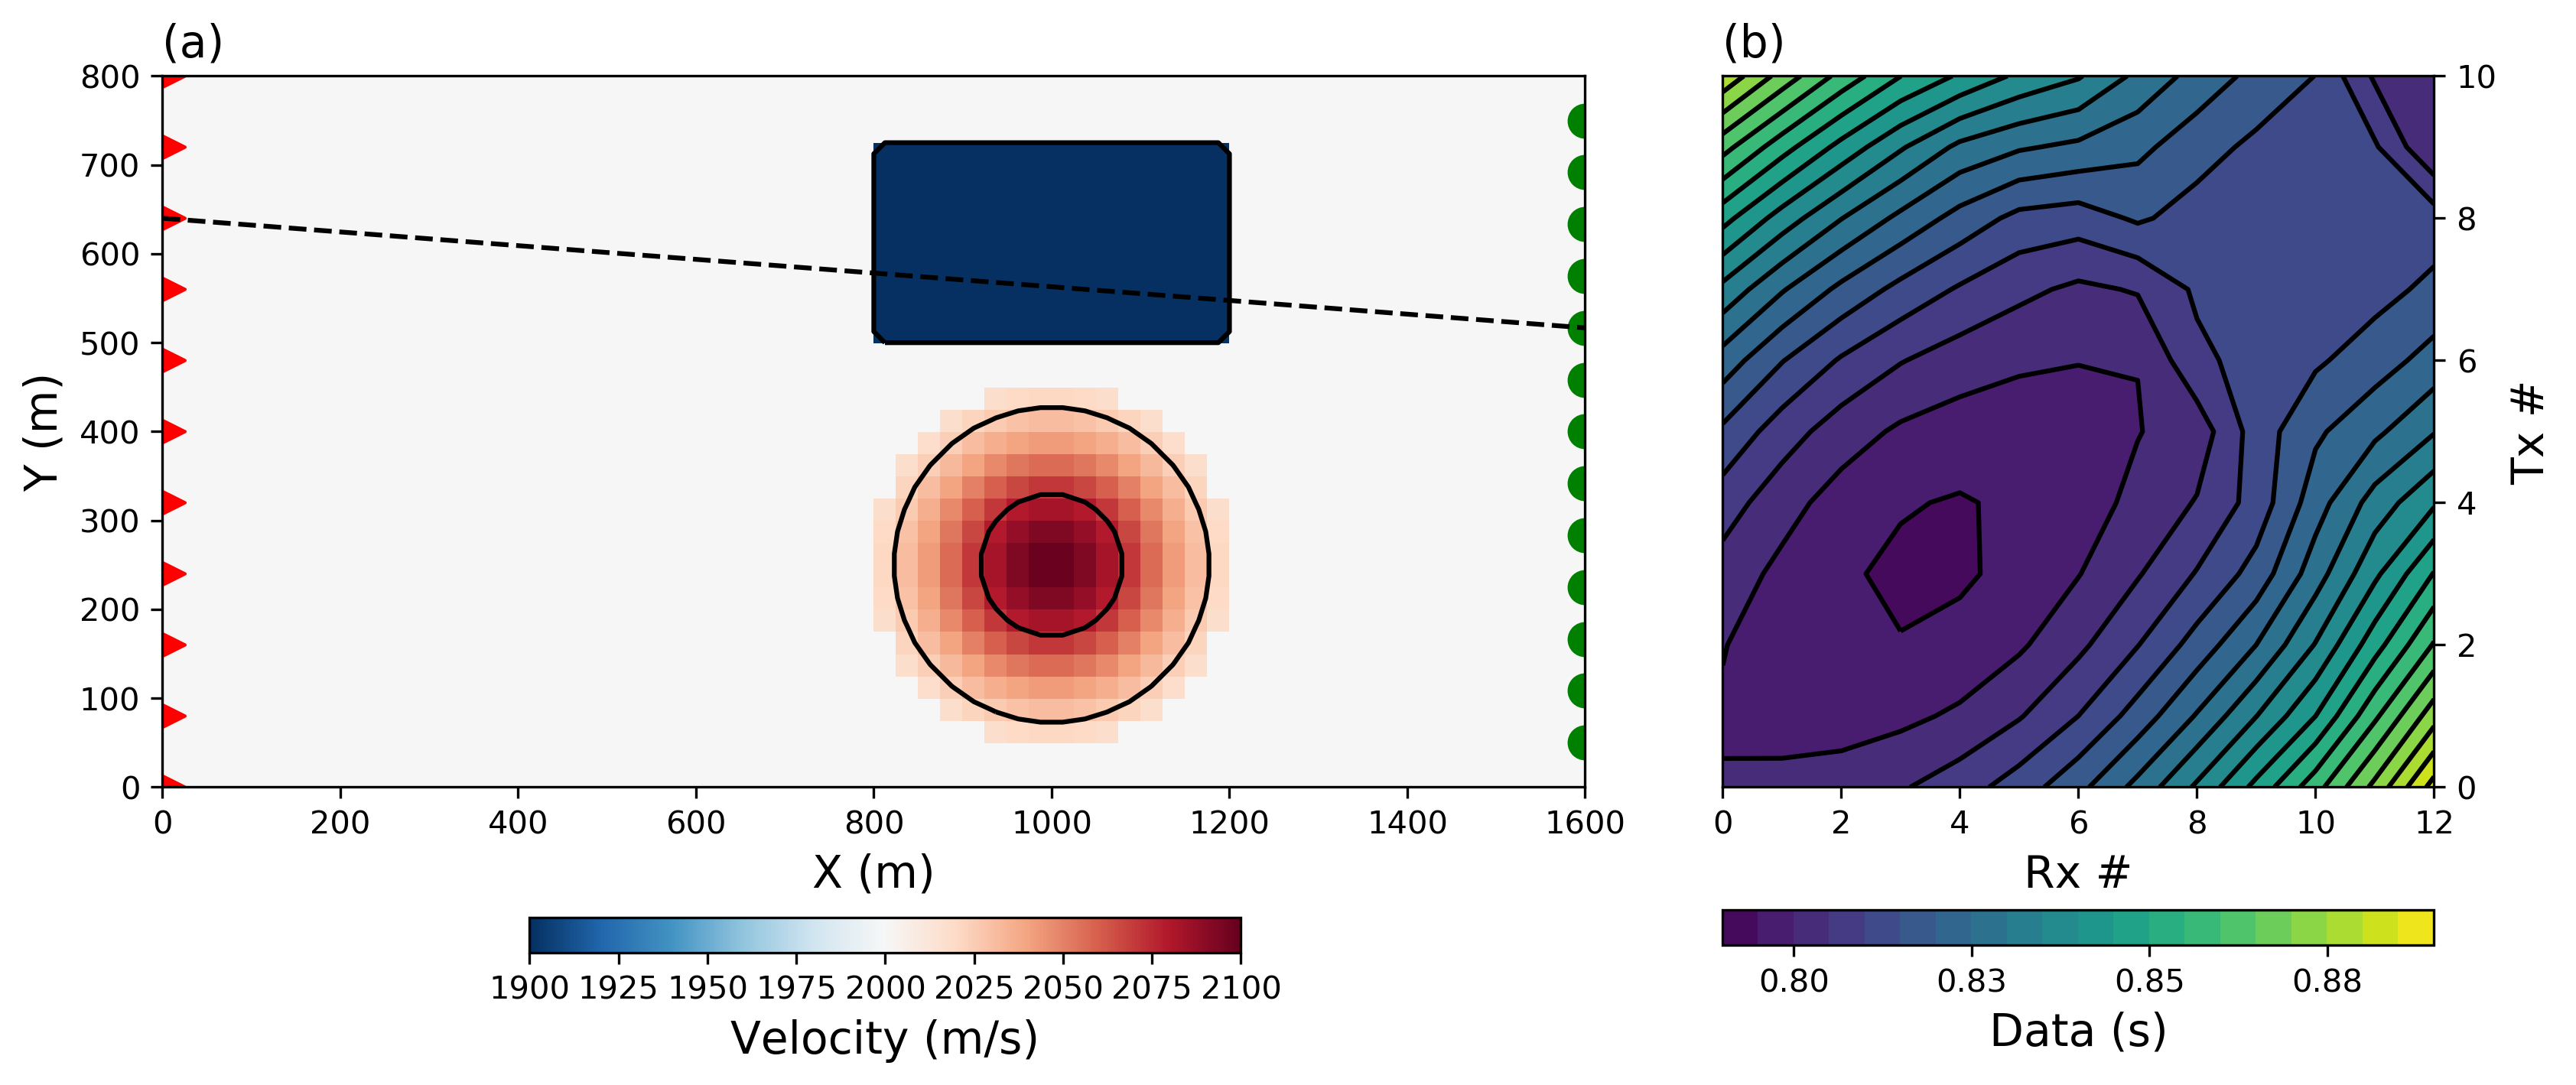
\includegraphics[width=\columnwidth]{Figures/Problem2D_True.png}
\caption{(a) Synthetic 2D travel-time tomography problem made up of a rectangular velocity low, and a smooth Gaussian velocity high. Contour lines ($25^{th}$ and $75^{th}$ percentile) are shown in black for the true position and shape of the velocity anomalies. Transmitters (red) and receivers (green) are positioned on opposite sides of the model domain. (b) Data map for the 143 line integral data calculated for each transmitter-receiver pair.
}
\label{Problem2DTrue}
\end{figure}


\subsubsection{Stage 1: $\ell_2$-norm solution}
Starting with Stage 1, we first solve this inverse problem with the conventional $\ell_2$-norm regularization ($p_s=p_x=p_y=2$). After convergence of the algorithm ($\phi_d \approx \phi_d^*$), we recover the model presented in Figure~\ref{Problem2D_l2norm}(a).
We can distinguish two velocity anomalies at roughly the right depth with respect to the true model.
We note however that the shape and horizontal extent of both targets are poorly defined.
Anomalies are stretched along the straight-ray paths associated with the experiment.

Visually, the solution exhibits characteristics of remaining near the reference model  of $2000$ m/s  while also attempting to be smooth.
Numerical evaluation of the components of the regularization function for this solution yields:
\begin{align*}
\begin{split}
\alpha_s \phi_s &= 1.23 \times 10^{-5}\\
\alpha_x \phi_x &= 1.34 \times 10^{-6}\\
\alpha_y \phi_y &= 7.04 \times 10^{-6}\;.
\end{split}
\end{align*}
This might suggest that $\phi_s$, $\phi_x$ and $\phi_y$ are roughly equal in importance.
As we later attempt to improve this solution with variable $\ell_p$-norm measures, we will need a general metric to evaluate our success in finding a solution in which components of the objective function have been equally influential.
Rather than comparing the actual values of the norms, we propose to quantify the relative
importance of each term based on their partial derivatives, or gradients. From \eqref{gradPhi} we expect to find an optimal solution where the sum of the gradients vanishes, either because all components are equal to zero, or because multiple gradients have opposite signs. To quantify the size of the gradients we use the infinity-norm
\begin{equation}
\left\| \mathbf{g}_j \right\|_\infty = \left\| \frac{\partial \phi_j}{\partial \mathbf{m}} \right\|_\infty
\end{equation}
The $\left\|\mathbf{g}_j \right\|_\infty$ metric is appealing for a few reasons: (a) it is directly linked to the minimization process because we use gradient descent methods, (b) it does not depend on the dimension $M$ of the parameter space as do other measures that involve a sum of components of the vector, (c) the theoretical maximum can be calculated analytically for any given $\ell_p$-norm function. These properties will become useful in the following section when we attempt to balance different norm penalties applied on a cell-by-cell basis.

We quantify the relative importance of the regularizations terms with a proportionality ratio:
\begin{equation}\label{derivRatio}
\lambda_\infty = \frac{ \alpha_s \left\|\mathbf{g}_s \right\|_\infty}{\alpha_x \left\| \mathbf{g}_x \right\|_\infty + \alpha_y \left\| \mathbf{g}_y \right\|_\infty}
\end{equation}
For the $\ell_2$-norm solution presented in Figure~\ref{Problem2D_l2norm}, we calculate a proportionality ratio near unity ($\lambda_\infty = 1.65$). This confirms that, with the current $\alpha$-scaling strategy, smallness and smoothness penalties are contributing near equally to the solution.
As we further generalize the regularization function for arbitrary $\ell_p$-norm measures, we will attempt to maintain this proportionality ratio ($\lambda_\infty \approx 1$) between competing functions.
From Figure~\ref{Problem2D_l2norm} we conclude that the $\ell_2$-norm regularization applied uniformly to the entire model domain does not provide an acceptable solution. We want to find more compact solutions but that display both smooth and abrupt boundaries. We therefore employ more general $\ell_p$-norms.

\begin{figure}
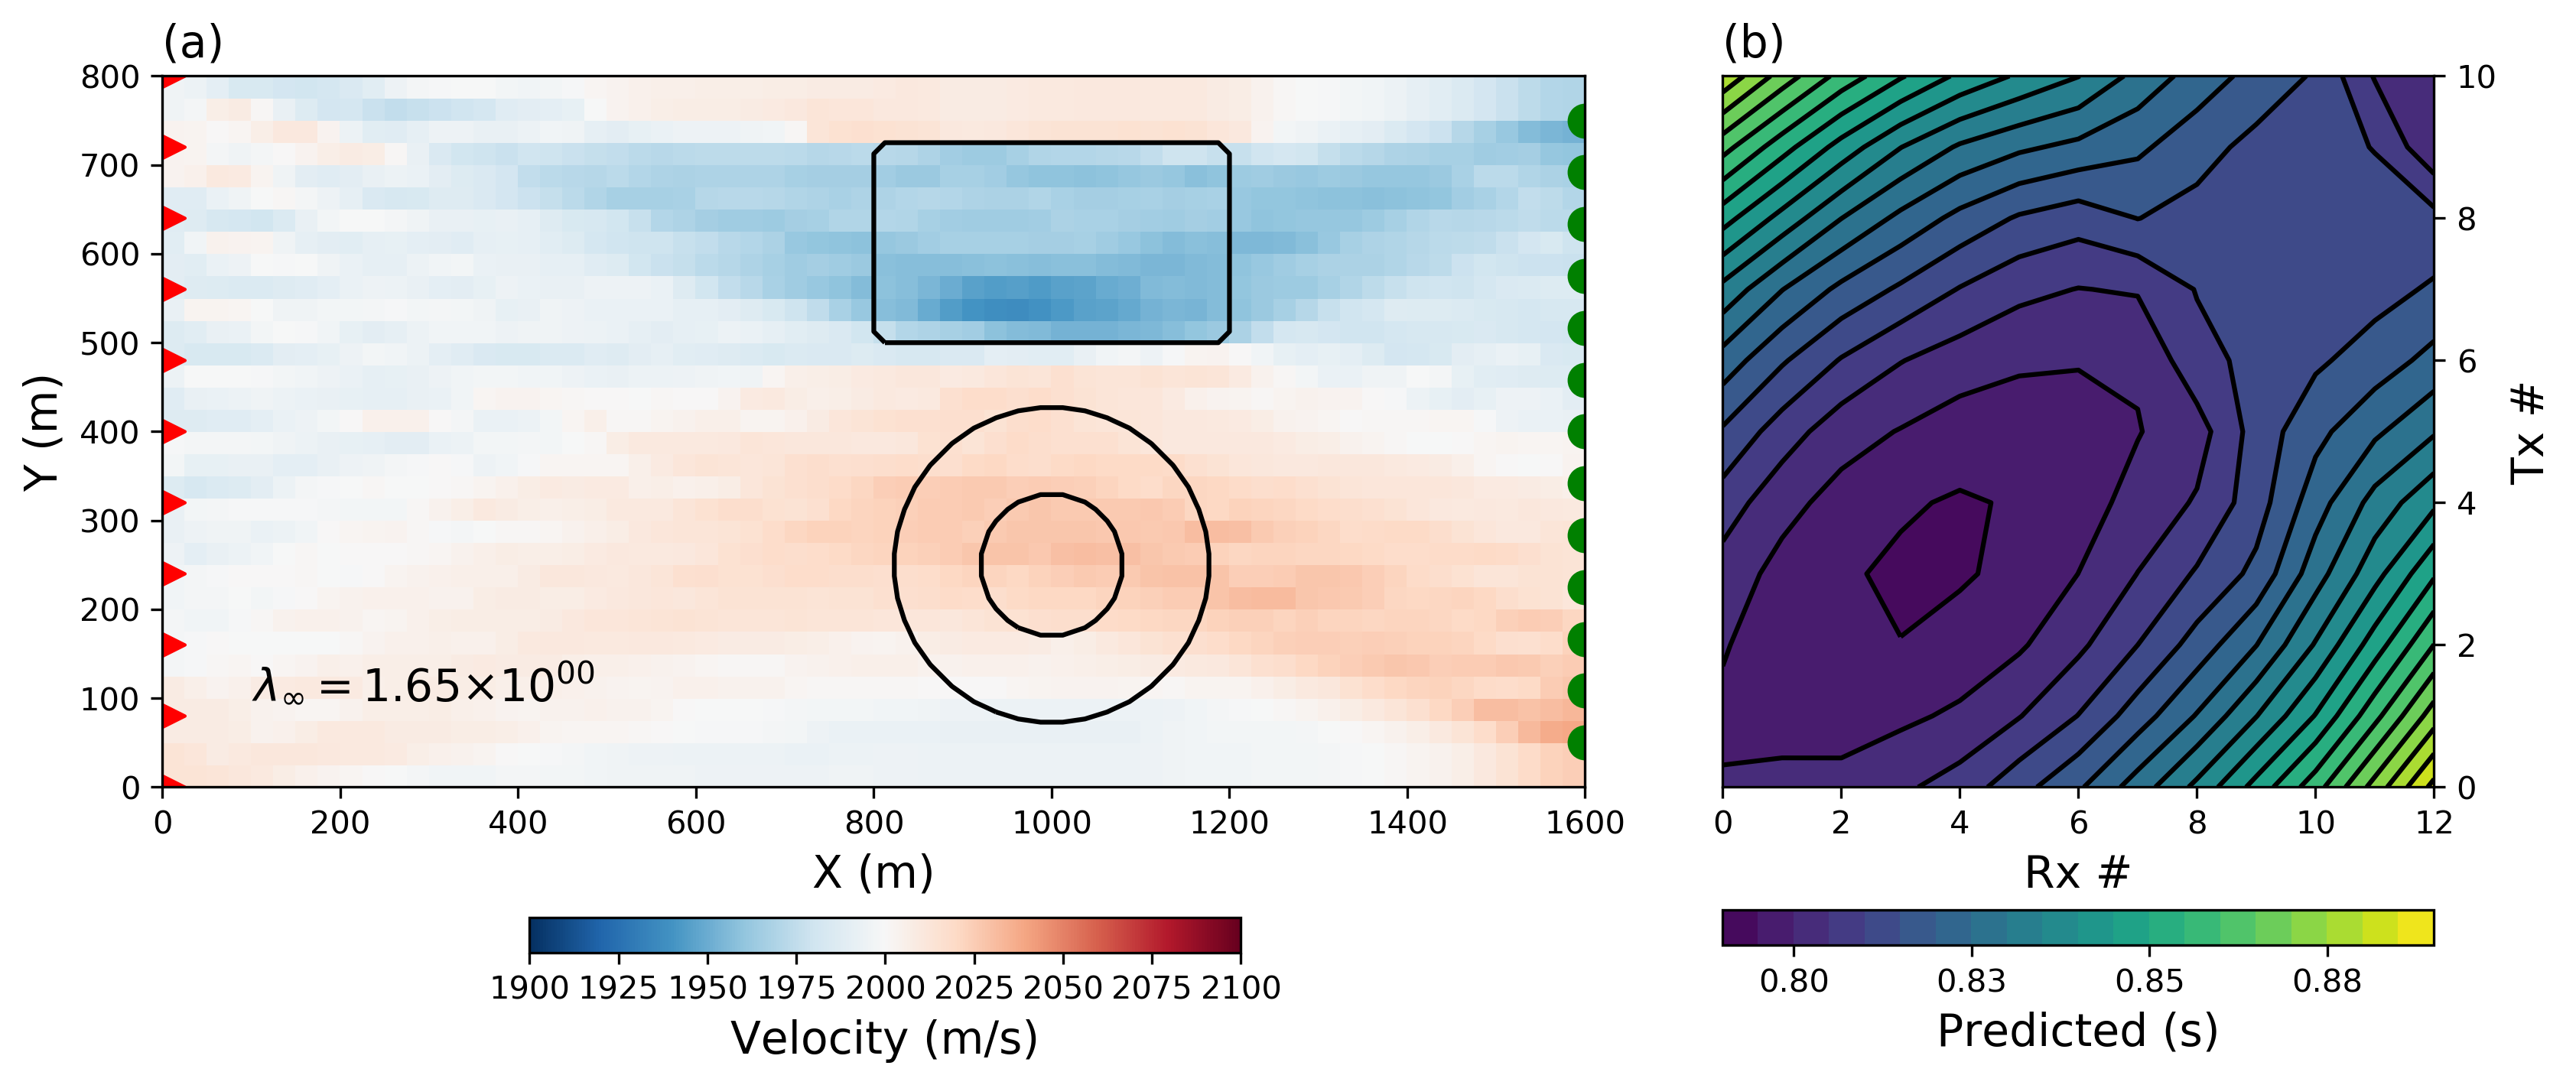
\includegraphics[width=\columnwidth]{Figures/Problem2D_l2Solution.png}
\caption{(a) Recovered smooth model and (b) predicted data. Contour lines are shown in (a) for the true position and shape of the velocity anomalies.
}
\label{Problem2D_l2norm}
\end{figure}


\subsubsection{Stage 2: $\ell_p$-norm penalties}

The idea of combining different norms for the simultaneous recovery of smooth and blocky features has partially been explored by \citet{SunLi14}. They demonstrated the benefits of dividing model space into regions with different $\ell_p$-norm penalties. The choice of norms was limited to be either $l_1$ or $l_2$-norm.
Little has been published however on the independent mixing of model and gradient norms on the range $p \in [0,2]$, although this problem was initially addressed in \cite[]{Fournier2015}.

Before attempting to vary the penalties locally (i.e. within the model domain) we first tackle the general mixed-norm problem.
As an entry point we attempt to minimize the following objective function:
\begin{equation}
\begin{split}\label{mixNorm}
\underset{\mathbf{m}}{\text{min}}\; \phi(m) & = \; \phi_d + \beta \left[ \alpha_s \phi_s^{\:0} + \sum_{j=x,y} \alpha_j \phi_j^{\:2} \right] \\
\text{s.t.} \; \phi_d & \leq \phi_d^* \; .
\end{split}
\end{equation}
Based upon our previous work, we expect the solution to be sparse, in terms of non-zero model parameters ($p_s = 0$), while smooth with respect to the model gradients ($p_x,\; p_y = 2$). This should be more suitable for  imaging smooth and compact velocity anomalies.
Using the standard IRLS strategy $(\alpha_s=\alpha_x=\alpha_y=1)$, we obtain the solution presented in Figure~\ref{Problem2D_lpnorm}(a). Instead of the expected smooth model we have recovered scattered anomalies concentrated near the velocity targets. The solution has been dominated by $\phi_s^{\:0}$. The influence from the smoothness penalties $\phi_x^{\:2}$ and $\phi_y^{\:2}$ has been marginal.
Comparing the partial derivatives of the objective function confirms this. After convergence, the calculated proportionality ratio is $\lambda_\infty = 7.31\times10^8$.
This is a significant change from the end of Stage 1 where $\lambda_\infty \approx 1$.
Clearly Stage 2 of the IRLS, took the solution away from the proportionality condition, which translated into the poor recovery of continuous velocity anomalies.

\begin{figure}
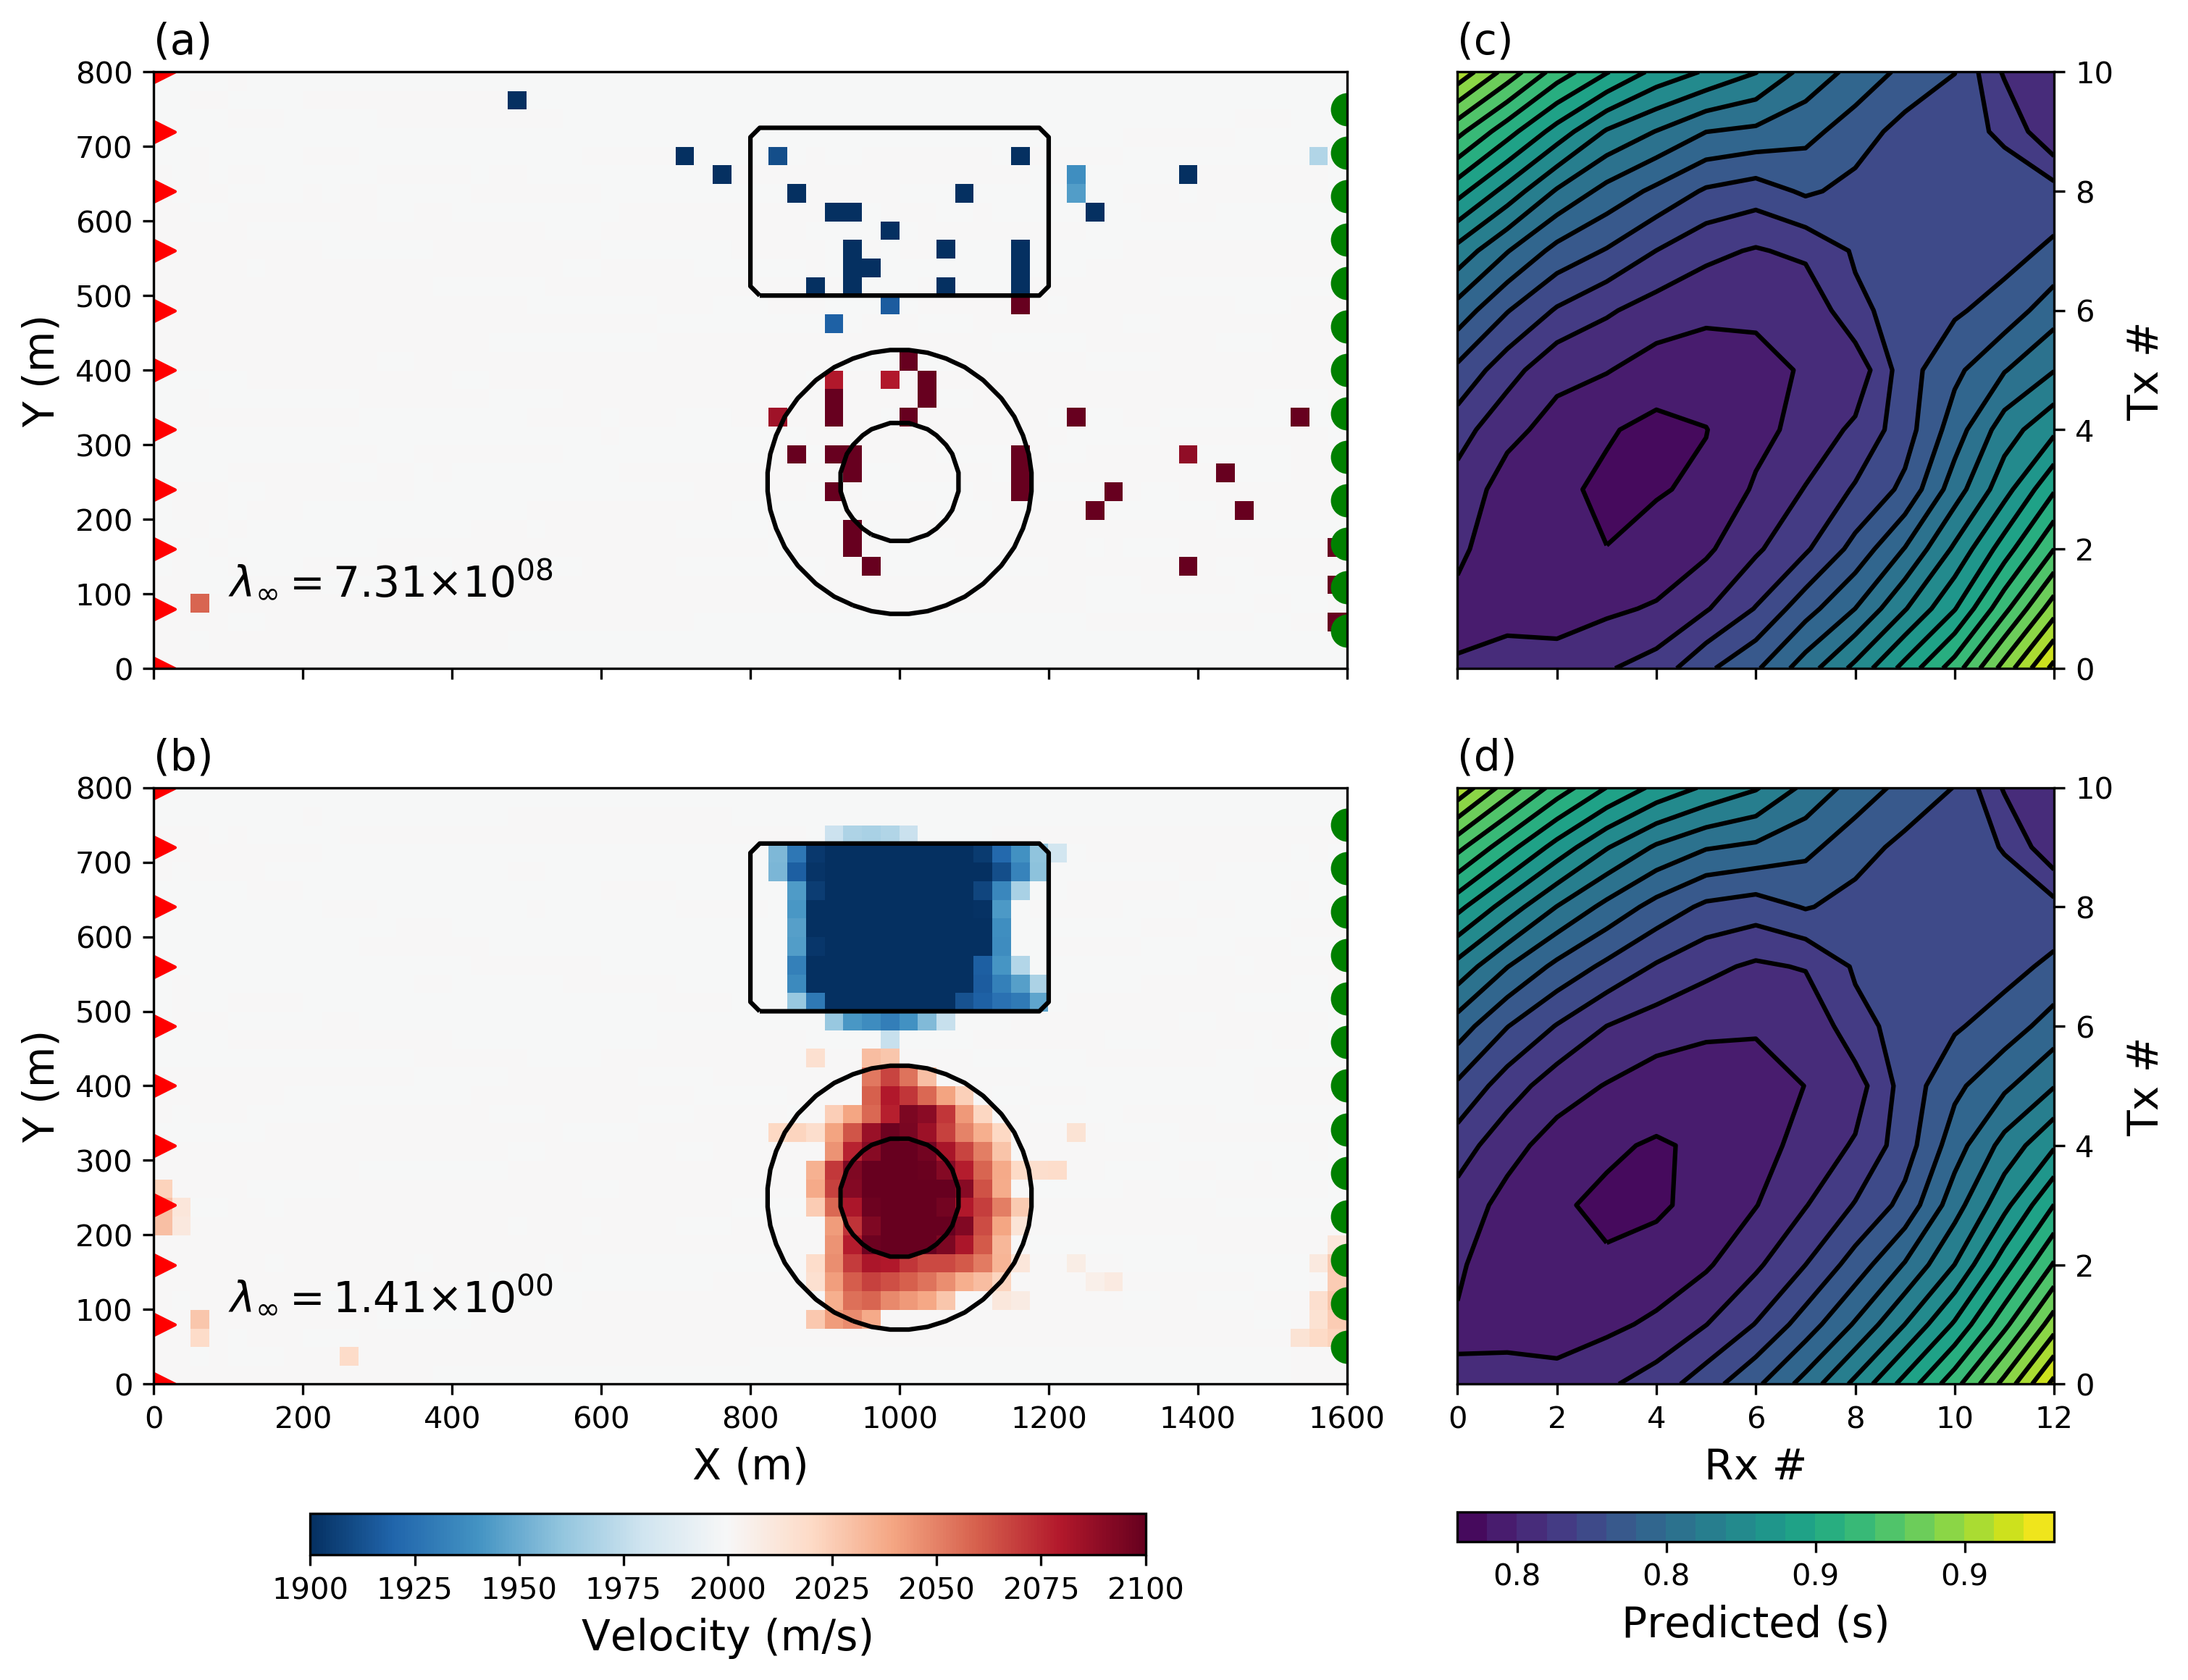
\includegraphics[width=\columnwidth]{Figures/Problem2D_MixedLpScale.png}
\caption{Recovered mixed-norm models using (a) the conventional IRLS and (b) the scaled-IRLS algorithm for $p_s=0$ and $p_x=p_y=2$. Contour lines are shown for the true position and shape of the velocity anomalies. (c), (d) Predicted data plot obtained with both approaches.
}
\label{Problem2D_lpnorm}
\end{figure}

\subsubsection{Scaled $\ell_p$-norm penalties}
A more desirable solution can be obtained if proportionality among the components of the objective function is preserved throughout the IRLS process.
Since the inverse problem is solved using gradients of the composite objective function $\phi(\mathbf{m})$, the relative magnitude of the individual gradients is a driving force in controlling the iteration step in \eqref{GaussNewtStep}.
Taking the partial derivatives of the linearized Lawson norm as prescribed in \eqref{eq:IntegralIRLS} yields
\begin{equation} \label{eq:IRLS_Grad_generic}
{g}^{p} = \frac{\partial \phi^{p}}{\partial {m}} = \frac{f(m)}{{{({f(m)}^{2} + \epsilon^2 )}^{1-p/2}} }V\;.
\end{equation}
In \eqref{eq:IRLS_Grad_generic} the superscript $p$ on the gradient, $g^p$, refers to the associated $p$-value and is not to be interpreted as an exponential.
These are plotted in Figure~\ref{NormDeriv}(a) as a function of $f(m)$ and for various values of $p$. We note that the magnitude of the derivative increases rapidly for small $p$ and $\epsilon$ values as $f(m) \rightarrow 0$.
This property of the IRLS approximation is important because, when attempting to combine different norm penalties within the same objective function, there will be a systematic bias towards small $\ell_p$-norm penalties.
To circumvent this bias we define the following gradient-based scaling
\begin{equation}\label{gammaScale}
\gamma = \left[\frac{\|g^2\|_\infty}{\|g^p\|_\infty}\right]^{1/2}
\end{equation}
By using this scaling we can equalize the size of the gradients associated with any $\ell_p$ -norm.
We can easily compute $\|g^p\|_\infty$ for any function $f(m)$ by taking the partial derivative of \eqref{eq:IRLS_Grad_generic} and setting it to zero. This maximum gradient of the Lawson approximation occurs at ${f(m)^*}$
\begin{equation}\label{mMaxGrad}
f(m)^* =
\begin{cases}
\infty \;\text{or}\; f(m)_{\text{max}},& p \geq 1 \\
\frac{\epsilon}{\sqrt{1-p}} ,&p < 1 \;,
\end{cases}
\end{equation}
from which we can calculate $\|g^p\|_\infty$ by substituting ${f(m)^*}$ into \eqref{eq:IRLS_Grad_generic}.
Figure~\ref{NormDeriv}(b) presents the scaled gradients for different approximated $\ell_p$-norms. Note that the largest derivative of any norm is at most as large as the $\ell_2$-norm penalty for $f(m) \in \mathbb{R}$. This equalization of the norm derivatives guarantees that multiple penalties can co-exist and impact the solution at every step of the IRLS, regardless of the chosen $\{p,\epsilon\}$-values.

\begin{figure}
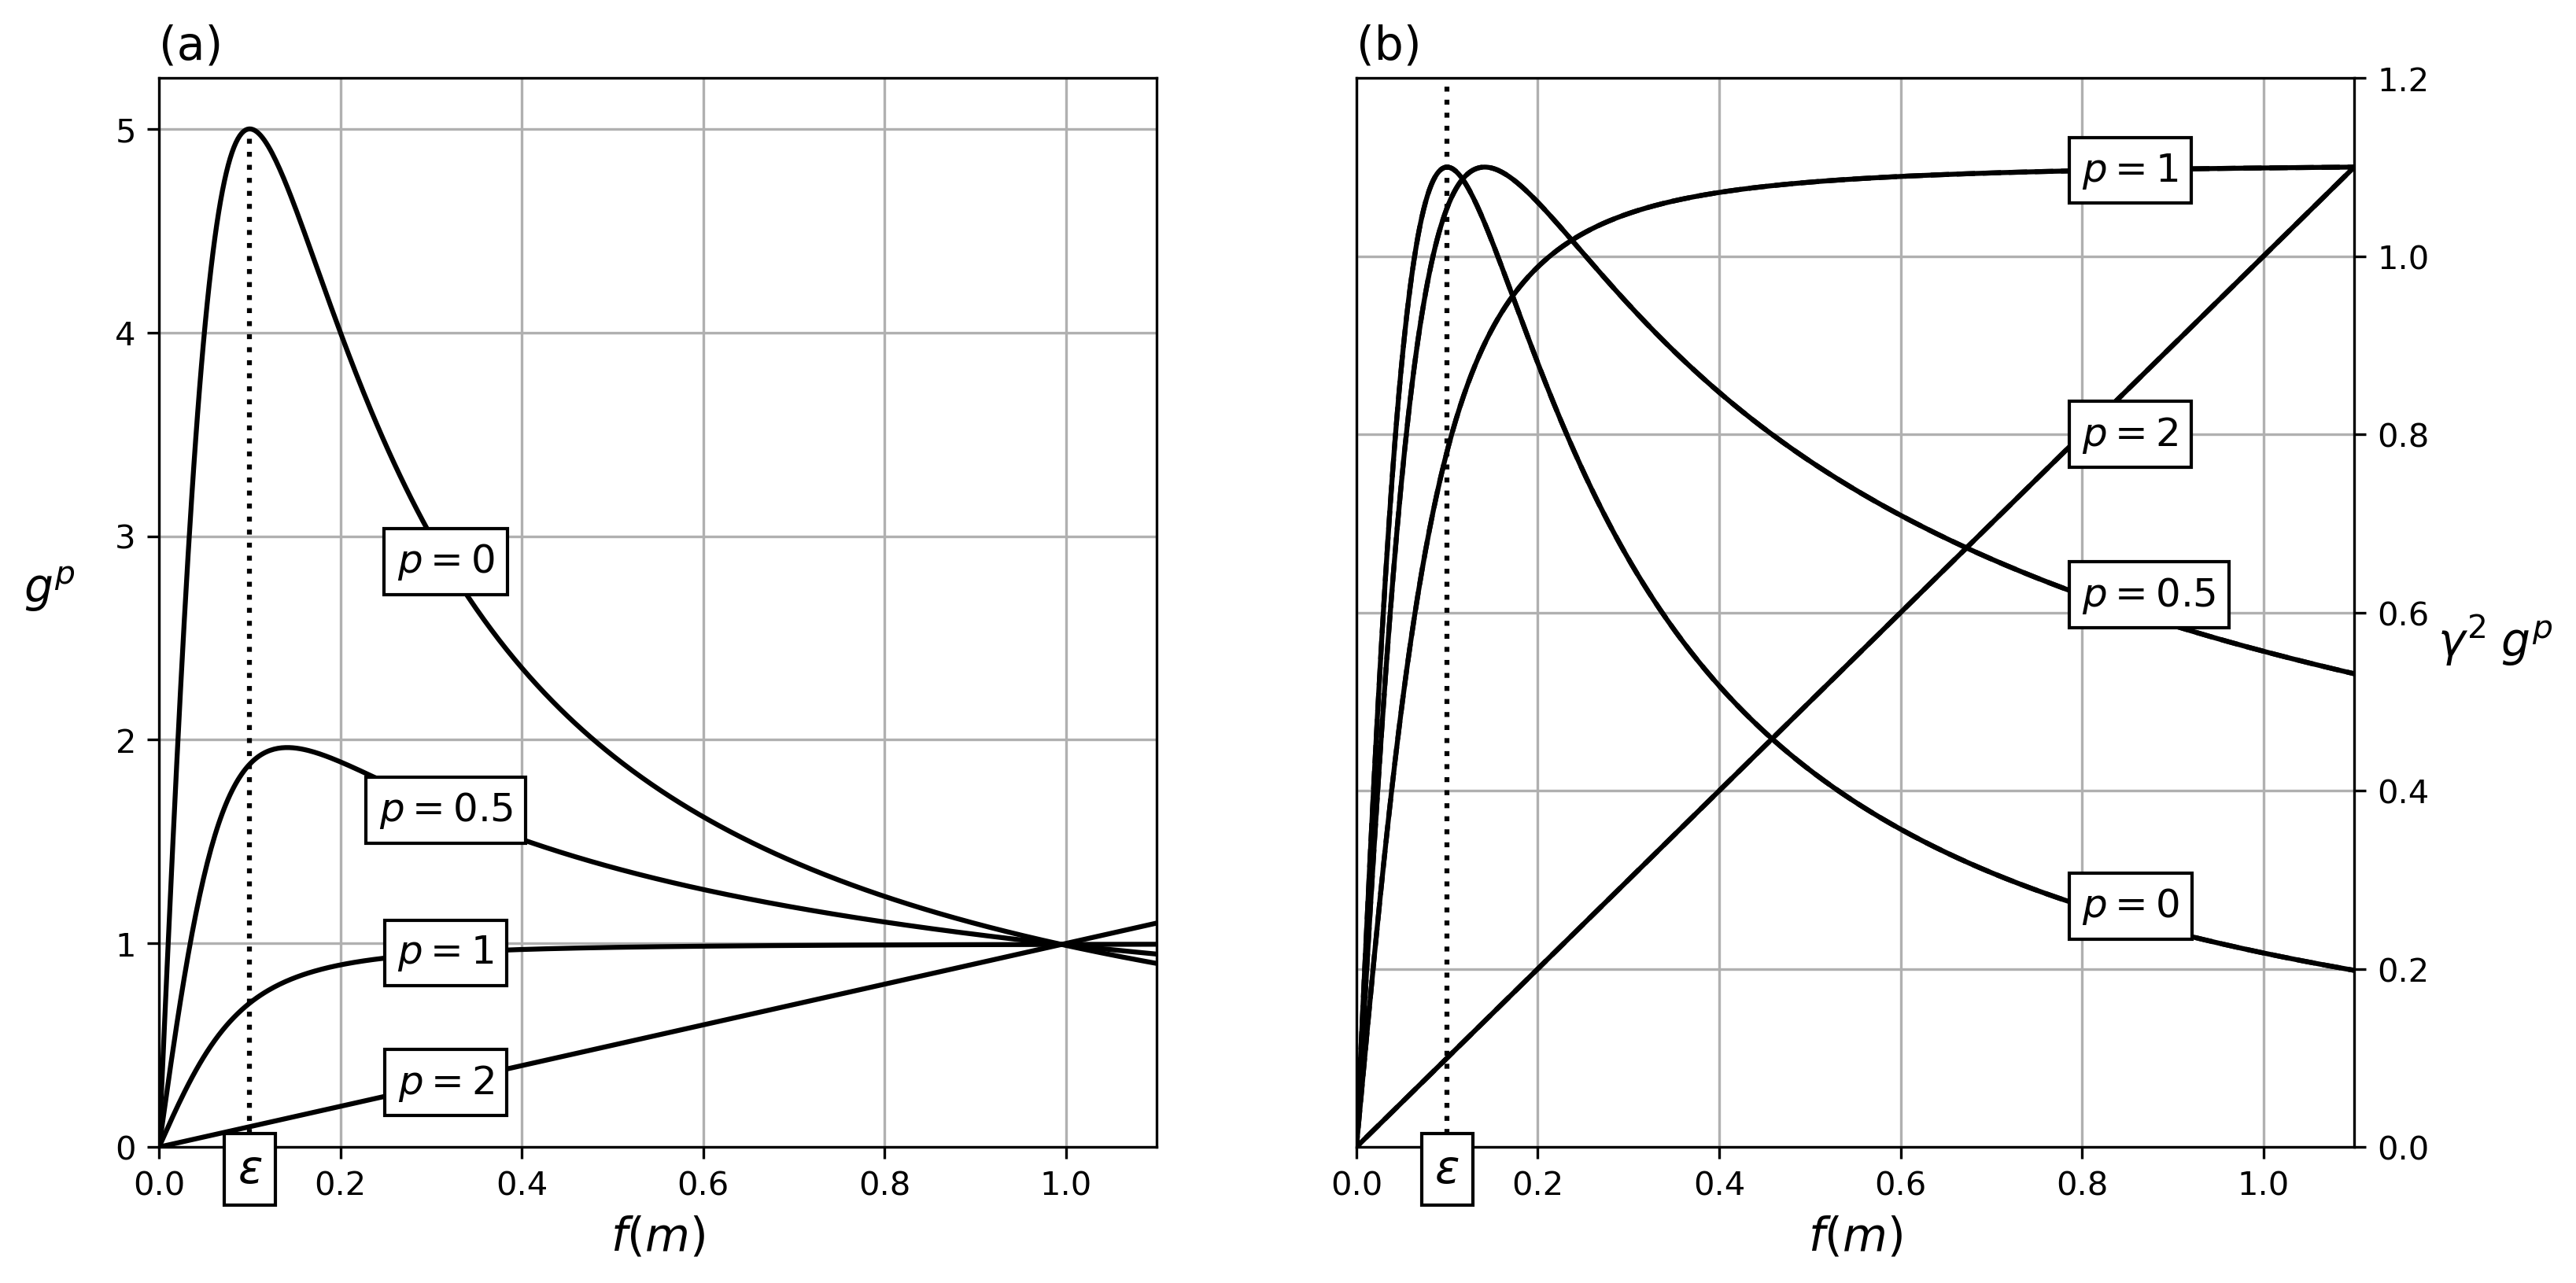
\includegraphics[width=\columnwidth]{Figures/NormDeriv.png}
\caption{(a) Derivatives of the Lawson approximation over range of model function $f(m)$ and for a fix threshold parameter $\epsilon=10^{-1}$, chosen for visual purpose only. For $p<2$, gradients increase rapidly as $f(m) \rightarrow 0$ resulting in a regularization function dominated by sparse norms. (b) Gradients after applying the $\gamma$-scaling, bringing all maximums to be equal.}
\label{NormDeriv}
\end{figure}

By applying the scaling  to the vector gradients of the model and derivatives term, we define a Scaled-IRLS (S-IRLS) regularization function of the form:
\begin{equation}\label{scaledIRLS1D}
\hat \phi^p_m = \alpha_s \| \mathbf{V}_s\:\mathbf{\hat R}_s\; \mathbf{m}\|_2^2 + \sum_{j=x,y,z} \alpha_j\|\mathbf{V}_j\:\mathbf{\hat R}_j\:\mathbf{D}_j\; \mathbf{m}\|_2^2
\end{equation}
such that IRLS weights in \eqref{eq:R_w} and \eqref{eq:Rx_w} are replaced by:
\begin{equation}\label{etaScale}
\begin{split}
\mathbf{\hat R}_s &= \gamma_s\; \mathbf{R}_s \\
\mathbf{\hat R}_j &= \gamma_j\; \mathbf{R}_j \;,
\end{split}
\end{equation}
The scaling parameters $\gamma_s$ and $\gamma_j$ are:
\begin{equation}
\begin{split}
\gamma_s &= \left[\frac{ \left\| \mathbf{g}_s^2 \right\|_\infty}{\left\|\mathbf{g}_s^{p_s}\right\|_\infty}\right]^{1/2} \;,\; \gamma_j = \left[ \frac{ \left\|\mathbf{g}_j^2\right\|_\infty}{\left\|\mathbf{g}_j^{p_j}\right\|_\infty}\right]^{1/2},
\end{split}
\end{equation}
This re-scaling is done for two reasons. First, at the transition between Stage 1 and 2, it preserves the balance between the misfit and regularization terms and thus no large adjustment in the trade-off parameter $\beta$ is needed. Secondly, this ensures that proportionality between $\phi^0_s $ and $\phi^2_j$ is preserved during the $\ell_p$-norm inversion.

Two options are possible to compute the $\gamma$-scalings: (a) take the maximum absolute gradient directly from the gradient values in \eqref{eq:IRLS_Grad_generic}, or (b) calculate $\left\|\mathbf{g}_j^p\right\|_\infty$ analytically as prescribed in \eqref{mMaxGrad}. We have found that Option 2 is more stable since it is based upon a theoretical maximum of the gradient and not on a particular realization of that maximum that arises from the distribution of values in the current model $\mathbf{m}^{(k)}$.

The outcome of the re-scaling strategy is shown in Figure~\ref{Problem2D_lpnorm}(b). The solution seems to have our desired properties of being sparse in terms of model values and having smooth edges. It is interesting to note from Figure~\ref{Problem2D_lpnorm}(c) and (d) that both solutions honor the observed data within the same tolerance, yet the S-IRLS solution is a better representation of the true model.
The final calculated proportionality ratio $\lambda_\infty = 1.41$ confirms that the scaling strategy was successful in balancing the impact of the sparse and smooth regularization functions.

\section{Automated mixed-norm modeling}
In the preceding section we have developed a methodology to find a solution that minimizes a combination of model norms. Different combinations of norms allow us to generate a variety of models that adequately fit the data and sample model space in a systematic manner.
This flexibility promotes two objectives.
First, inverting for diverse models provides immediate insight about non-uniqueness and can prevent practitioners from over-interpreting a single inversion result. This is one of the most important aspects of our work. The second objective is more challenging. As outlined in the introduction, we want to use different combinations of norms on different parts of the model space so that we obtain solutions that are geologically informative.
This selection process can rapidly become overwhelming for large problems in complex geological settings. A semi-automated approach that can capture the heterogeneity of the Earth, with minimal intervention from an expert, is needed. Our strategy is:
\begin{enumerate}
\item Run a suite of inversions over a range of $p$ parameters applied to the model norm and its spatial gradients. We will assume that the suit of models is a representative sampling of diverse solutions from the $\ell_p$-space.
\item Form an \emph{average} model ($\mathbf{m}_P$) that captures most of the variability in the solution space
\item Extract $p$ parameters for windowed portions of model space based on the correlation between the average $\mathbf{m}_P$ and individual models.
\item Carry out a final SVMN inversion with local $p$ parameters.
\end{enumerate}
There are numerous ways to implement the above strategy. Here, we use a combination of Principal Component Analysis and edge detection algorithms. We illustrate our approach with a 2D synthetic example and a 3D field example.

\subsection{Exploring the model space}
Having dealt with scaling issues between $\ell_p$-norm measures, we can now exploit the full flexibility of the regularization function in \eqref{intSmall}.
Our goal is to generate a suite of models under a broad range of assumptions.
To demonstrate the flexibility of our algorithm, we carry out seven additional inversions, using a combination of norms on a range of $p_s,\; p_{x},\;p_y \in {[0,1,2]}$ values ($p_x=p_y$ in all cases). The solutions, nine in total,  are presented in Figure~\ref{Mixed2DSolutions}. All models have a final misfit $\phi_d^* \approx 143$ and use the same $\ell_2$-norm solution to initiate the IRLS steps.
\begin{figure}
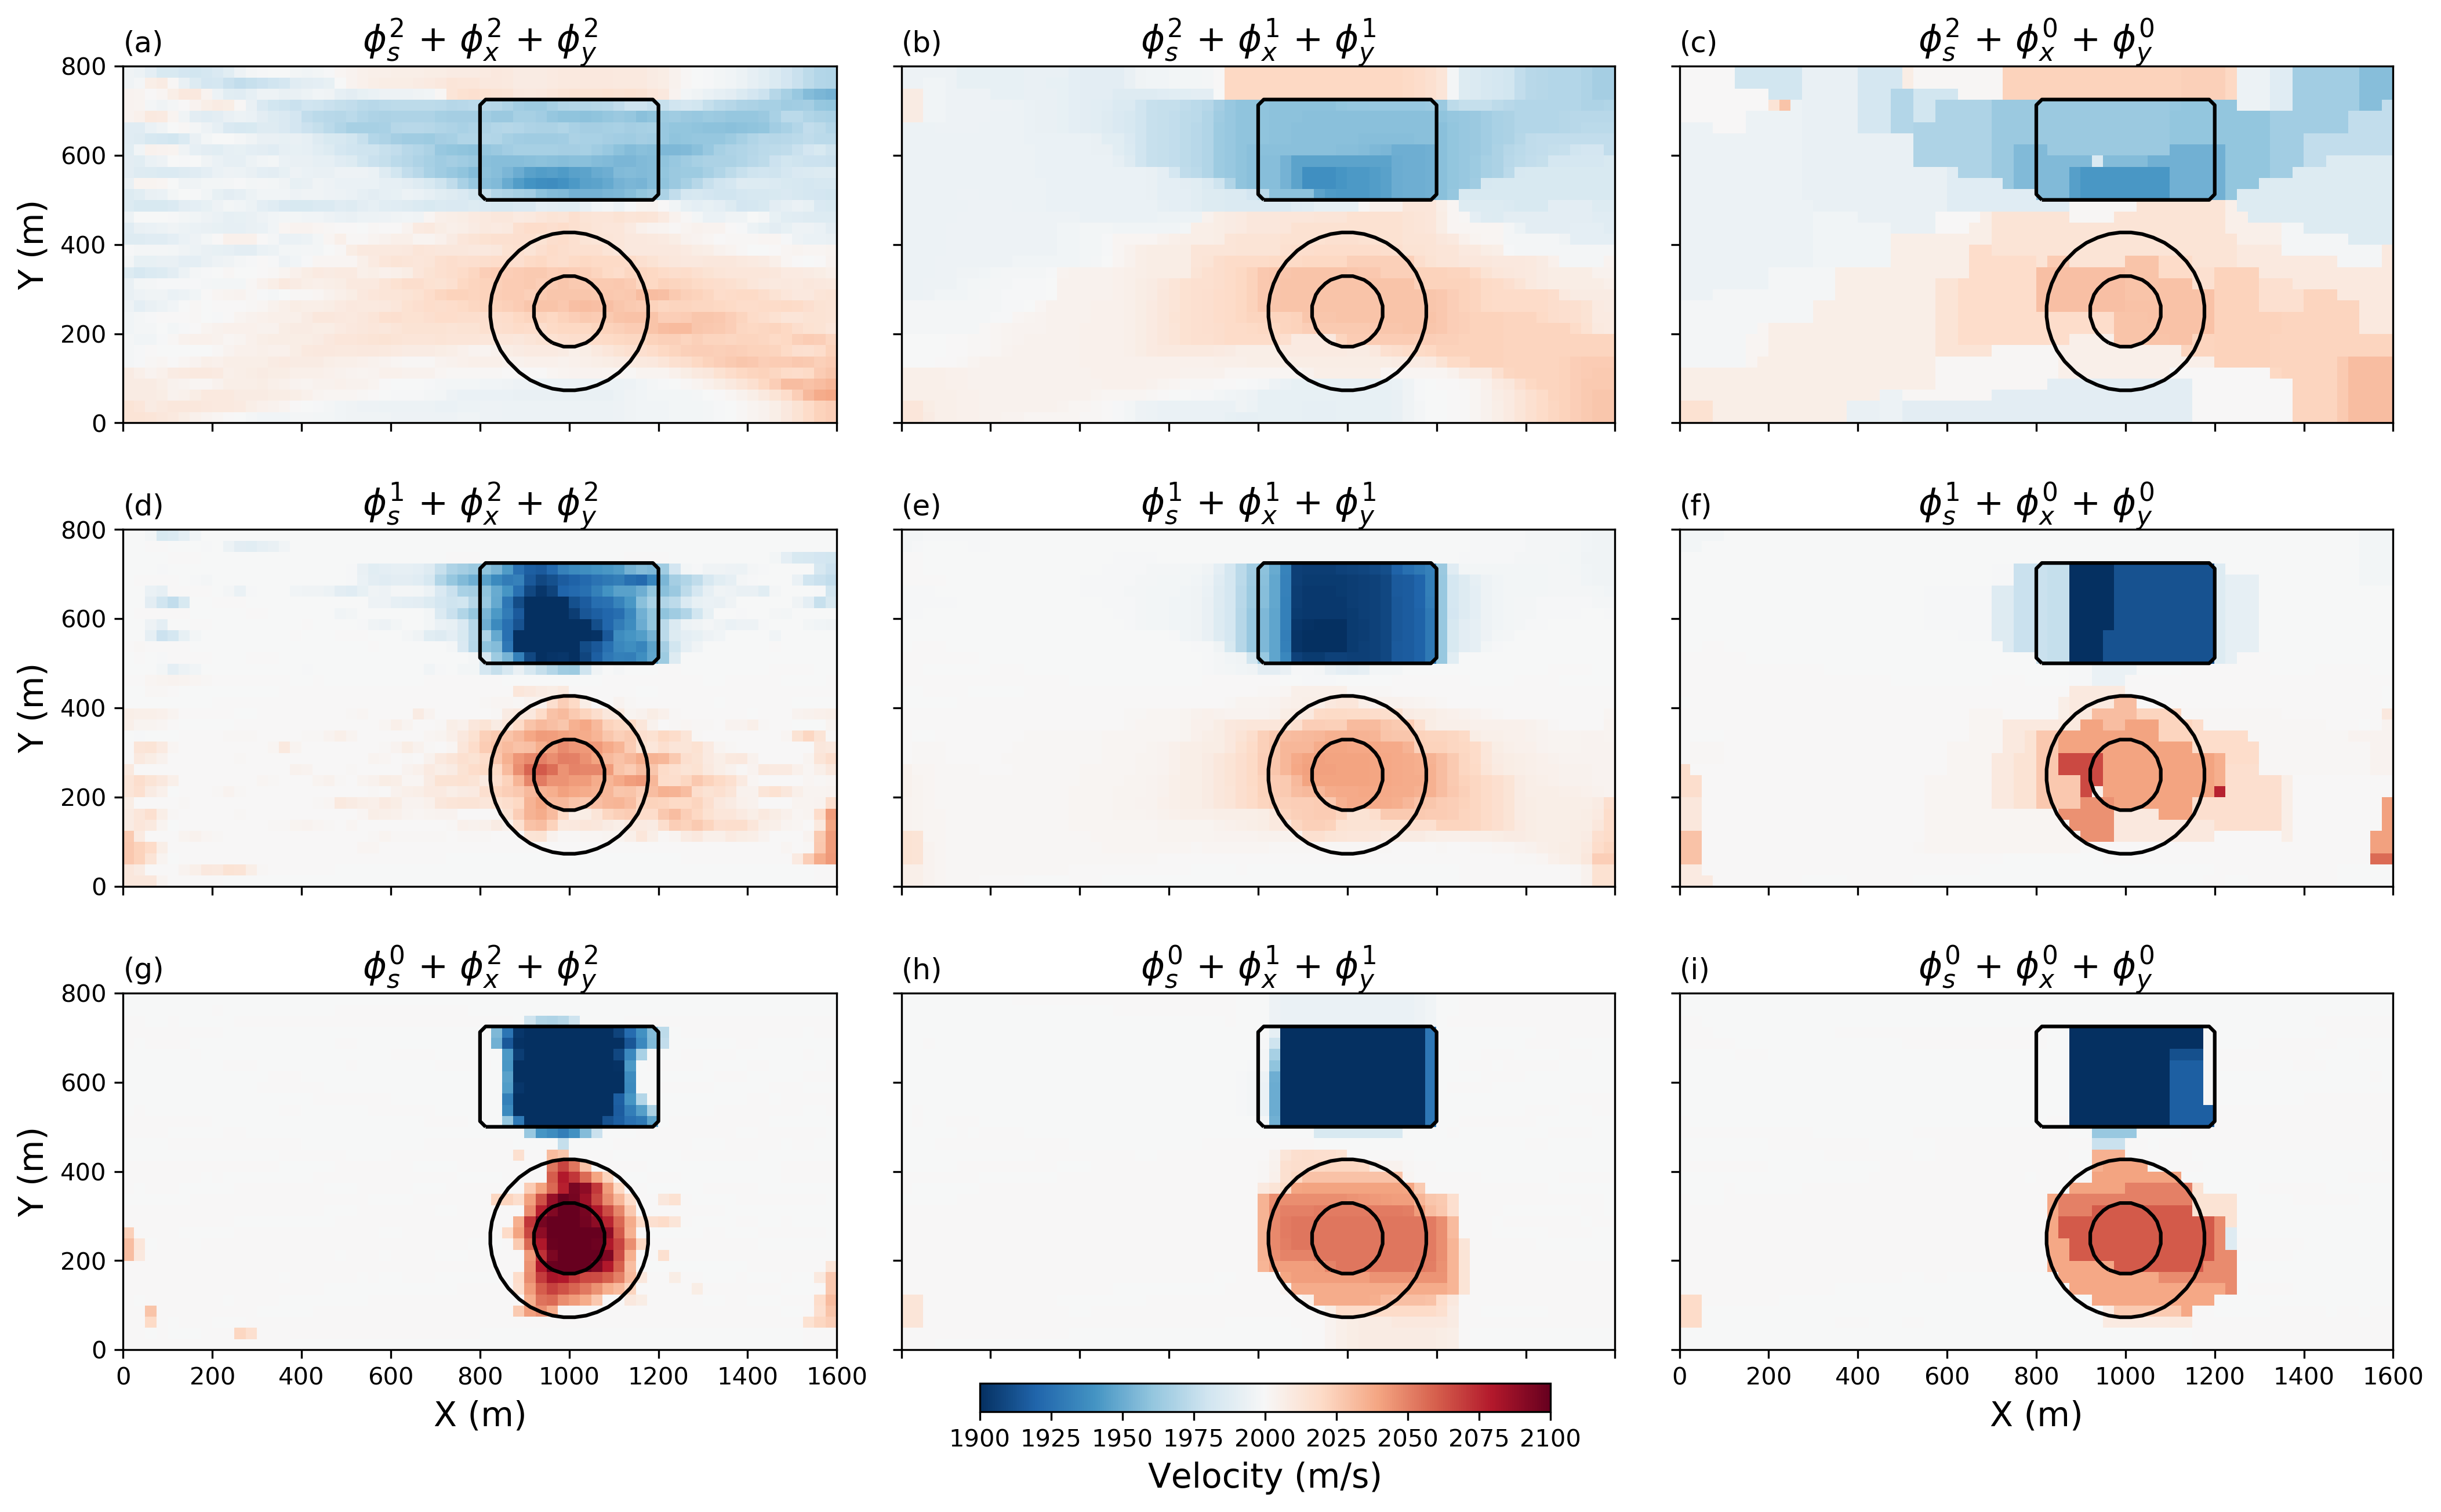
\includegraphics[width=\columnwidth]{Figures/Problem2D_Tomo2D_9x9_Results.png}
\caption{Suite of inverted models for various combination of norms $p_s,\; p_{x}=p_{y} \in {[0,1,2]}$ ($\alpha_s=\alpha_x=\alpha_y=1$). Contour lines ($25^{th}$ and $75^{th}$ percentile) are shown in black for the true position and shape of the velocity anomalies.}
\label{Mixed2DSolutions}
\end{figure}
We make the following observations. The two velocity anomalies centered at $1000$ m on the $x$-axis are dominant features. There is a progressive transition from a smooth model (upper left) to a blocky solution (lower right) as $p_s$, $p_{x}$ and $p_y$ decrease. The upper body (velocity low) appears to be most often represented as a blocky body with sharp edges. The lower anomaly (velocity high) tends to be more smooth. Away from the anomalous regions the velocity is relatively smooth and close to the background reference model of $2000$ m/s.


\subsection{Average PCA model}
We assume that the suite of models presented in Figure~\ref{Mixed2DSolutions} contains sufficient variability to be representative of our solution space and we wish to use these to extract the main features. There are numerous approaches to accomplish this and they vary in complexity from simple averaging to advanced machine learning algorithm.
We use a Principal Component Analysis \cite[]{Pearson1901, Hotelling1933}.
Considering each model in Figure~\ref{Mixed2DSolutions} as a \emph{data} vector, the principal components of our solution space can be written as:
\begin{equation}
\begin{bmatrix}
\mathbf{m}_1\;, ...\;, \mathbf{m}_{nM}
\end{bmatrix} \approx
\mathbf{A\:W}\;.
\end{equation}
such that PCA vectors along the columns of $\mathbf{A} \in \mathbb{R}^{nM \times nV}$ contains a subset of $nV$ eigenvectors spanning the model space. These vectors encode the principal source of variation across the nine models recovered.
The corresponding weights $\mathbf{W} \in \mathbb{R}^{nV \times nM}$, also known as loadings, are scalars relating how each principal component contributes to each model. We use the PCA algorithm from the open-source Python library \texttt{Scikit-Learn.decomposition.PCA} \cite[]{Pedregosa2011}. The number of principal components to be used in the analysis is determined by the experimenter.
Figure~\ref{PCA_vectors} presents the four largest principal components, covering in this case over $75\%$ of the variance present in the model space.

\begin{figure}
{\centering
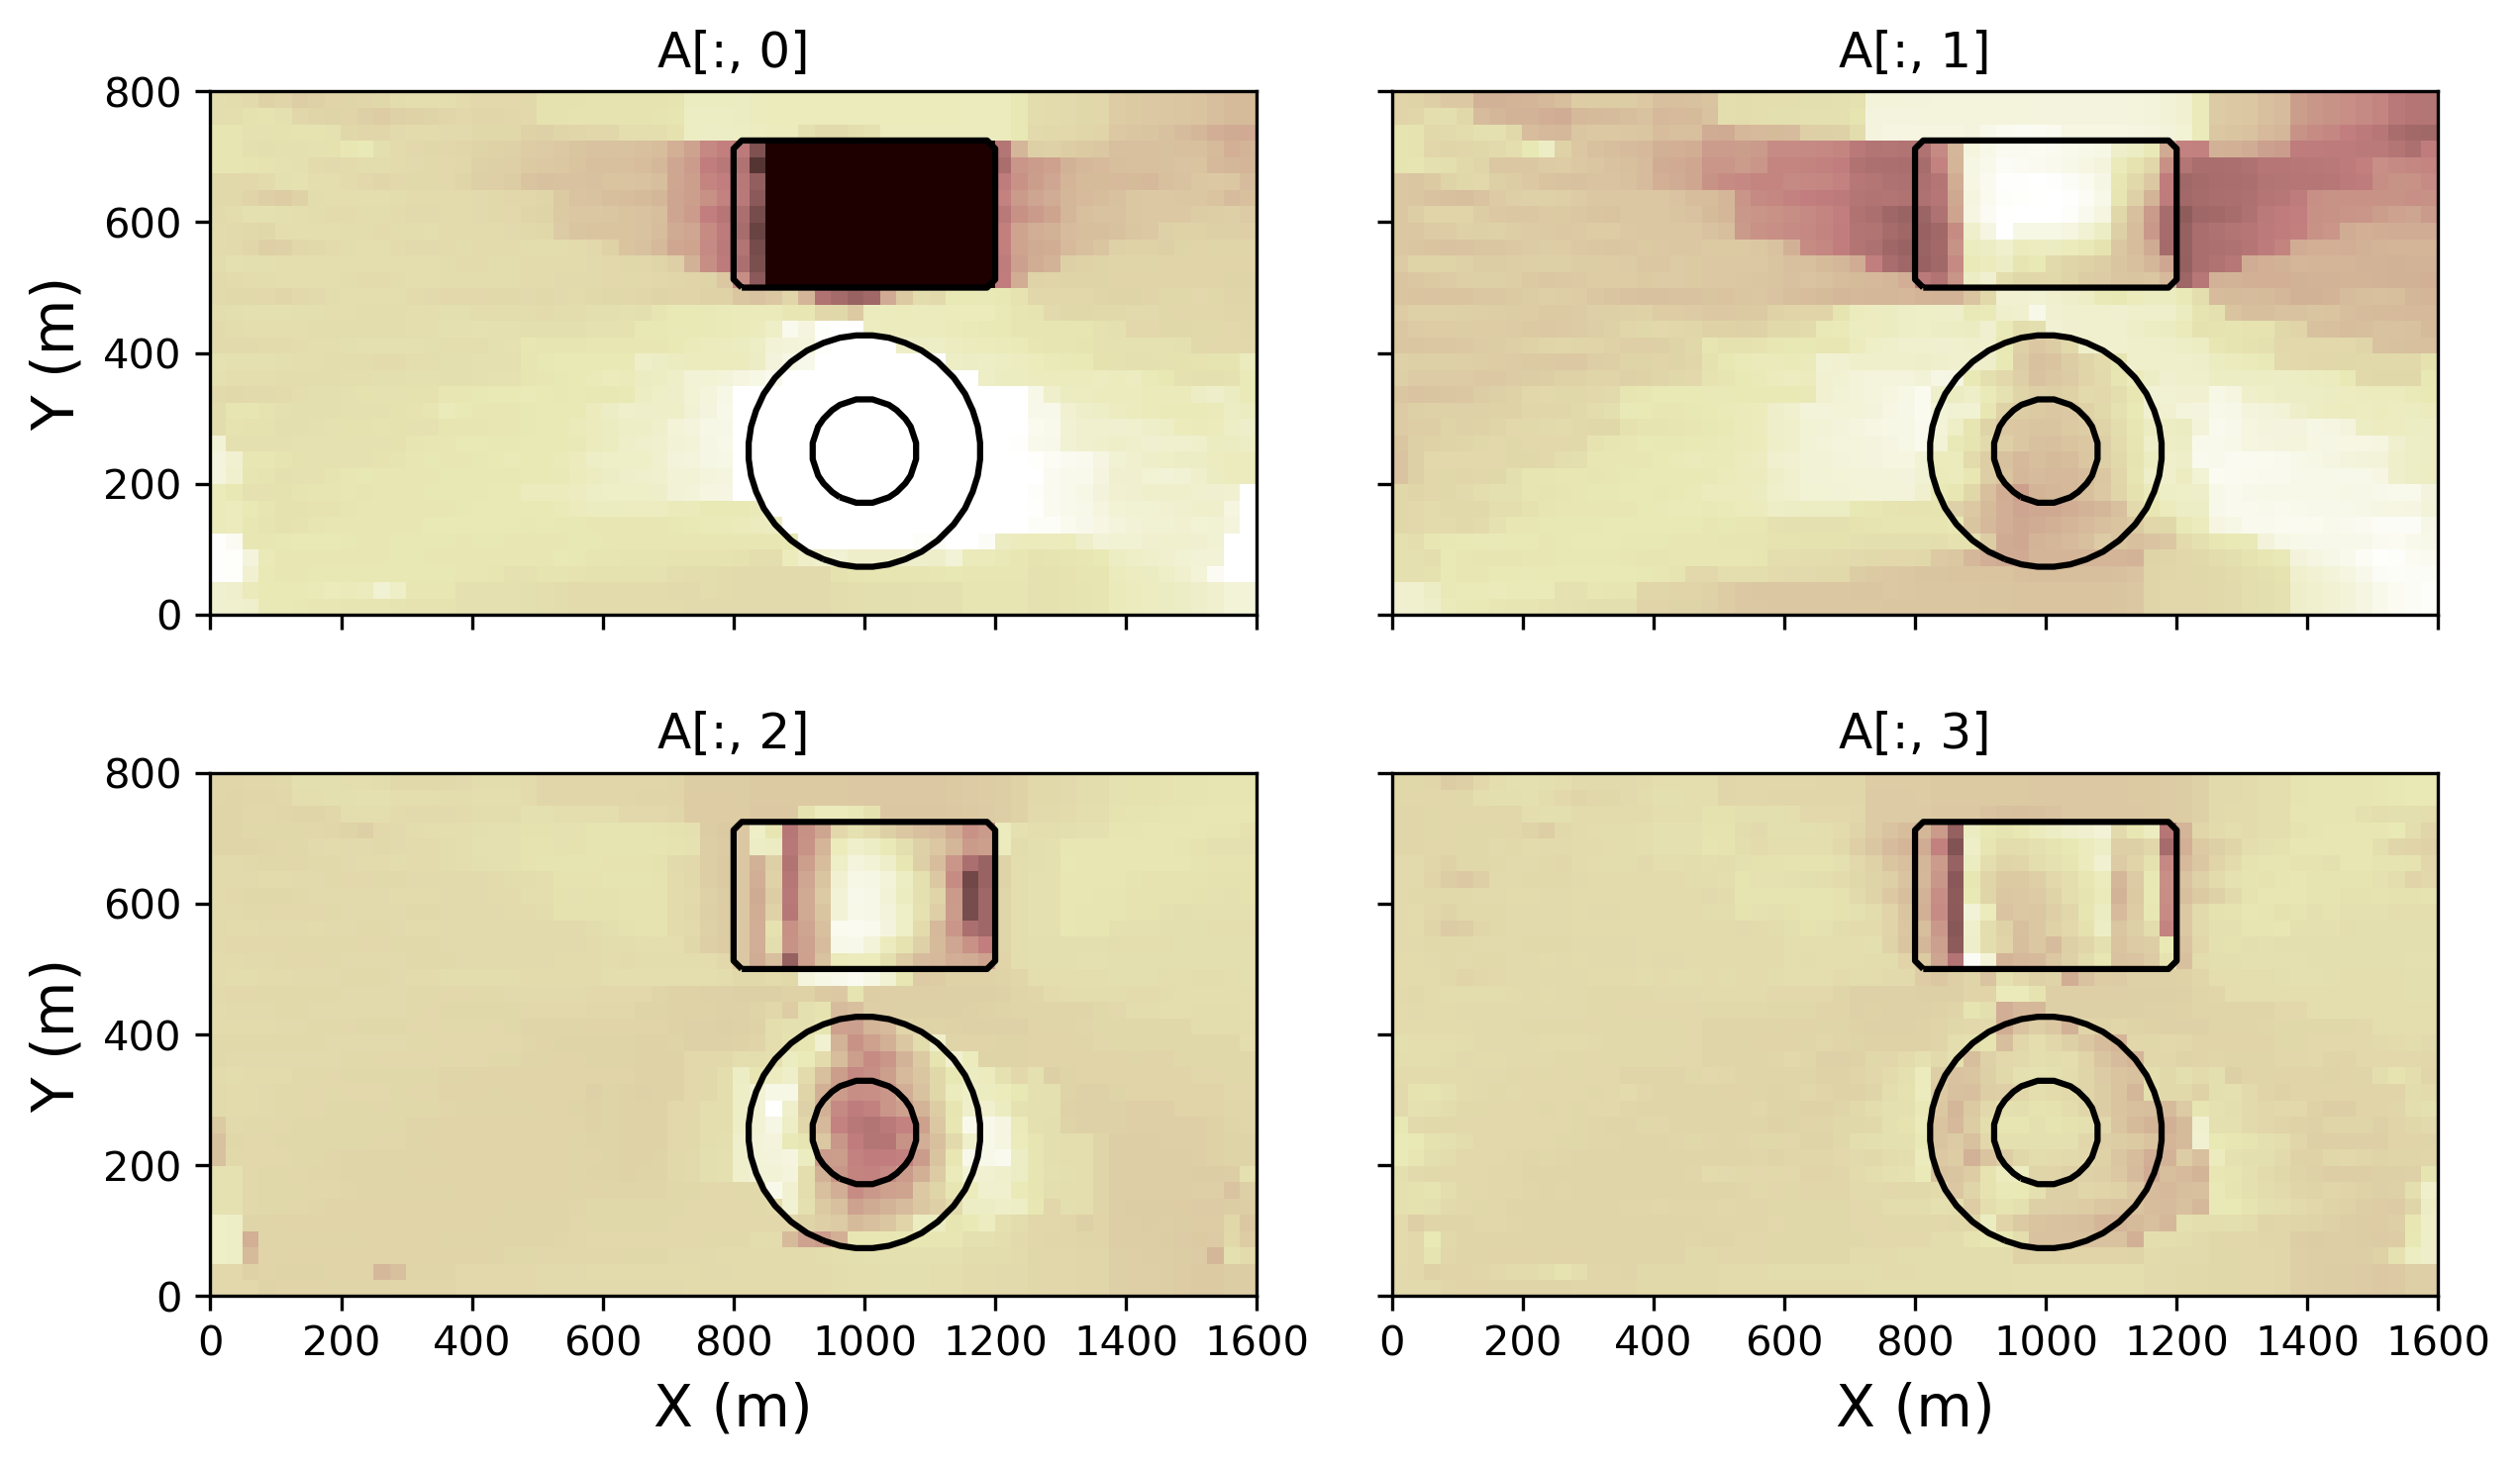
\includegraphics[width=\columnwidth]{Figures/Tomo2D_StackPCA.png}
\caption{PCA vectors covering $75\%$ of the model variances.}\label{PCA_vectors}}
\end{figure}
\begin{figure}
{\centering
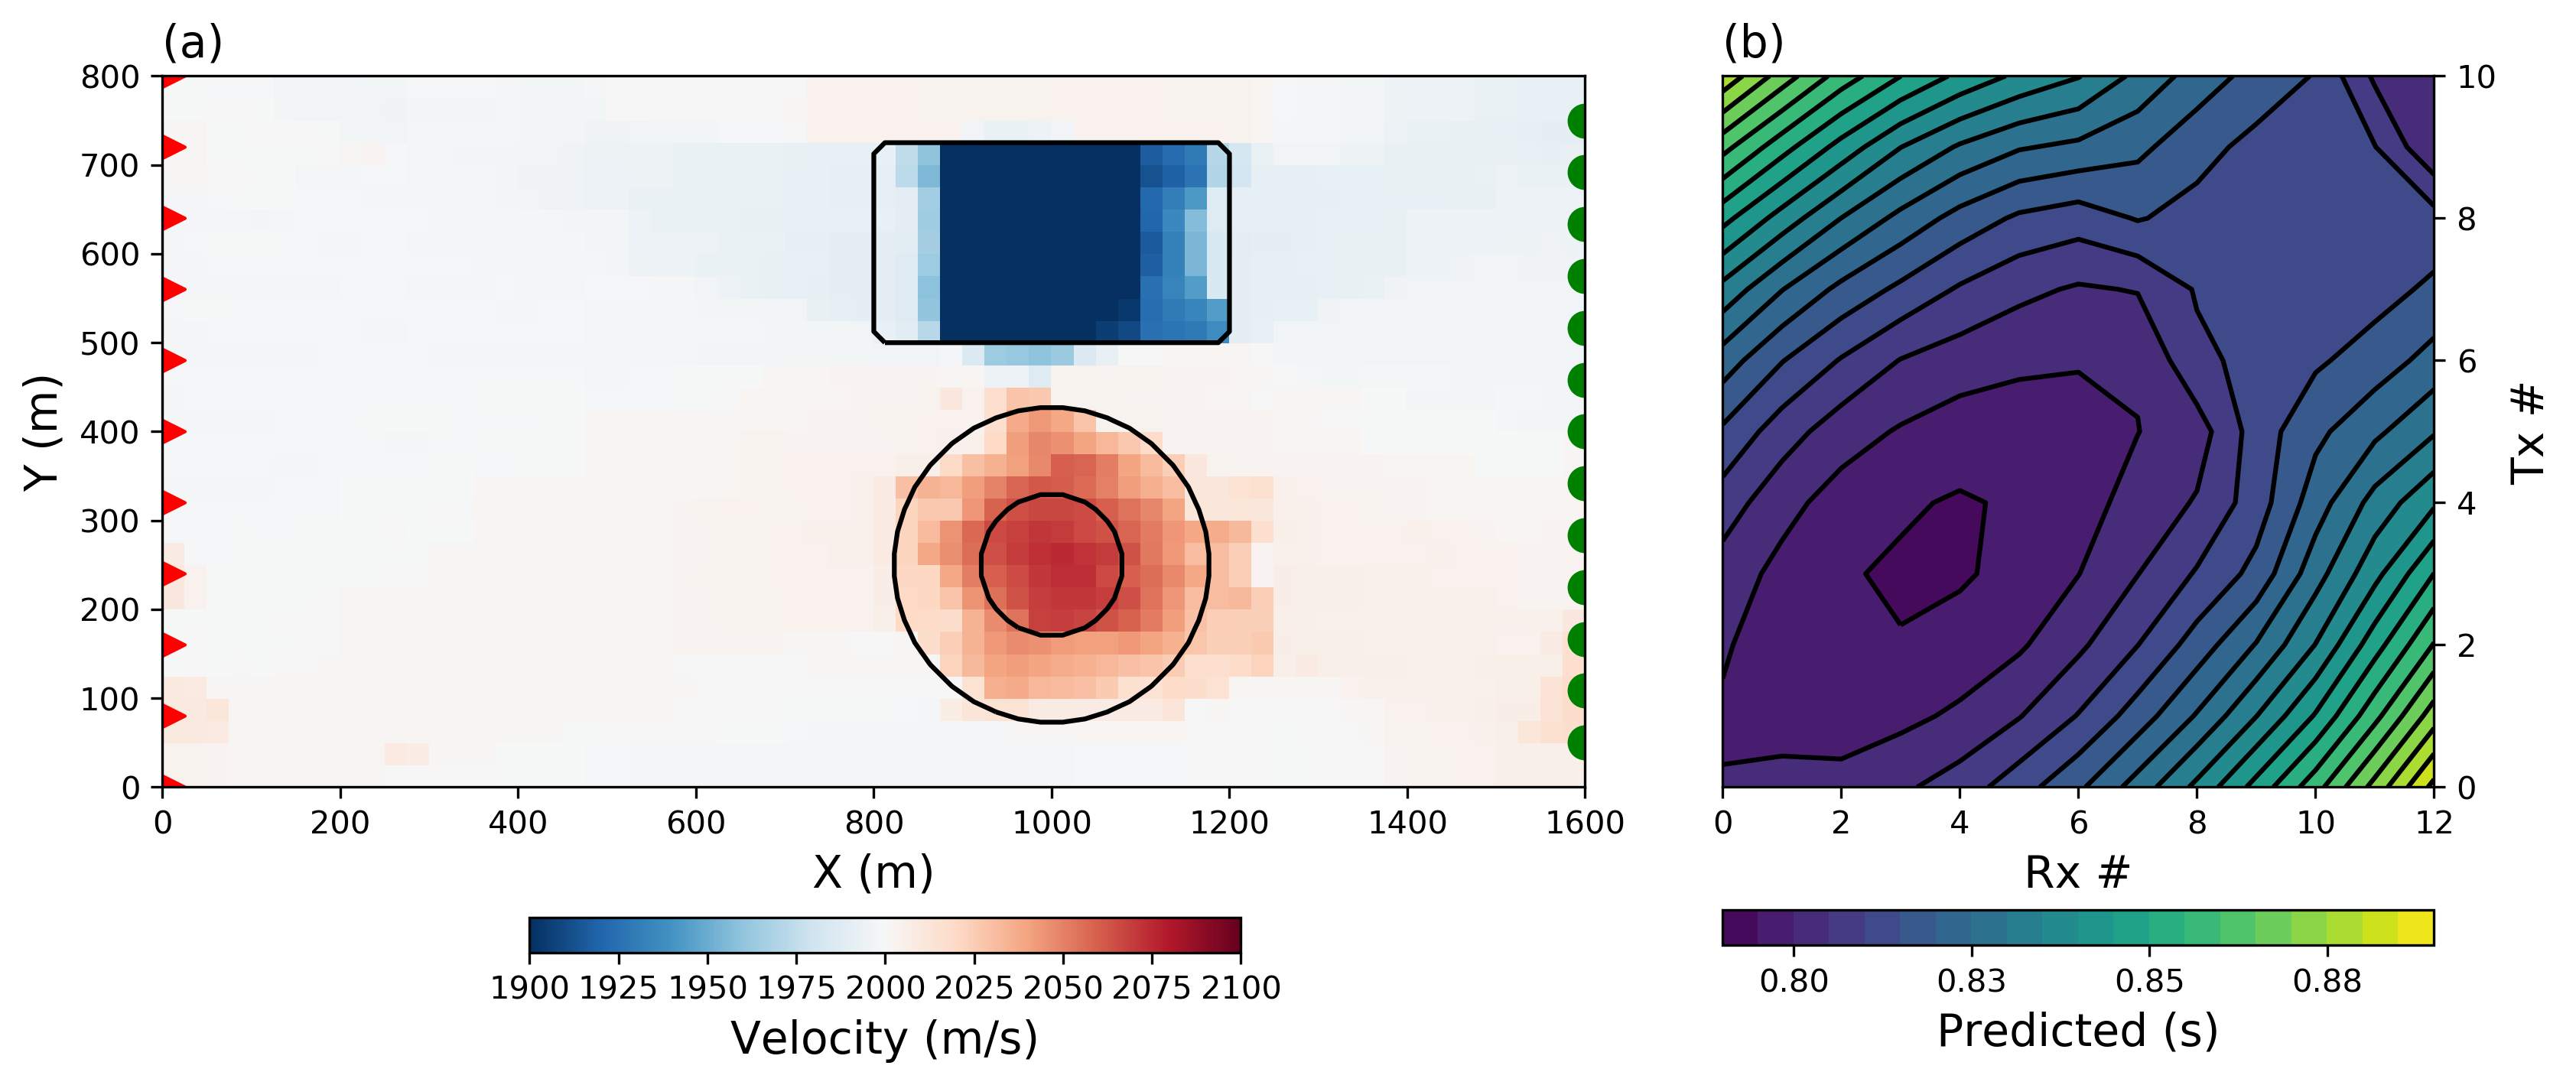
\includegraphics[width=\columnwidth]{Figures/Results_PCA_model.png}
\caption{(a) Averaged PCA model $\mathbf{m}_P$ (b) predicted data. Contour lines are shown in (a) for the true position and shape of the velocity anomalies.}\label{PCA_model}}
\end{figure}
Next, we generate a representative model by computing a weighted averaged model based on the positive PCA loadings such that:
\begin{equation}\label{weightedaverage}
\mathbf{m}_P = \frac{\sum_{i=1}^{nV} \sum_{j=1}^{nM} W_{ij} \mathbf{m}_i}{ \sum_{i=1}^{nV} \sum_{j=1}^{nM} W_{ij}} \;.
\end{equation}
The average model $\mathbf{m}_P$ is presented in Figure~\ref{PCA_model}. We note the close resemblance with the true model. The background is fairly uniform near $2000\;m/s$; the low velocity anomaly appears to be a block with a velocity near $1900\;m/s$, and the high velocity anomaly appears is a smooth feature with a maximum velocity near $2100\;m/s$.


\subsection{Parameters extraction}
Next, we want to extract optimal inversion parameters on a cell-by-cell basis in order to best describe local features. To do so, we resort to a pattern recognition approach. In order to remove biases towards extreme model values, we transform our model space into a simpler parametric representation. We use a Canny edge detection algorithm from the open-source library \texttt{Scikit-Image.feature.Canny} \cite[]{Pedregosa2011}.
Figure~\ref{CannyEdges} shows the parametric edges extracted from all nine inversions and the average PCA model $\mathbf{m}_P$
\begin{figure}
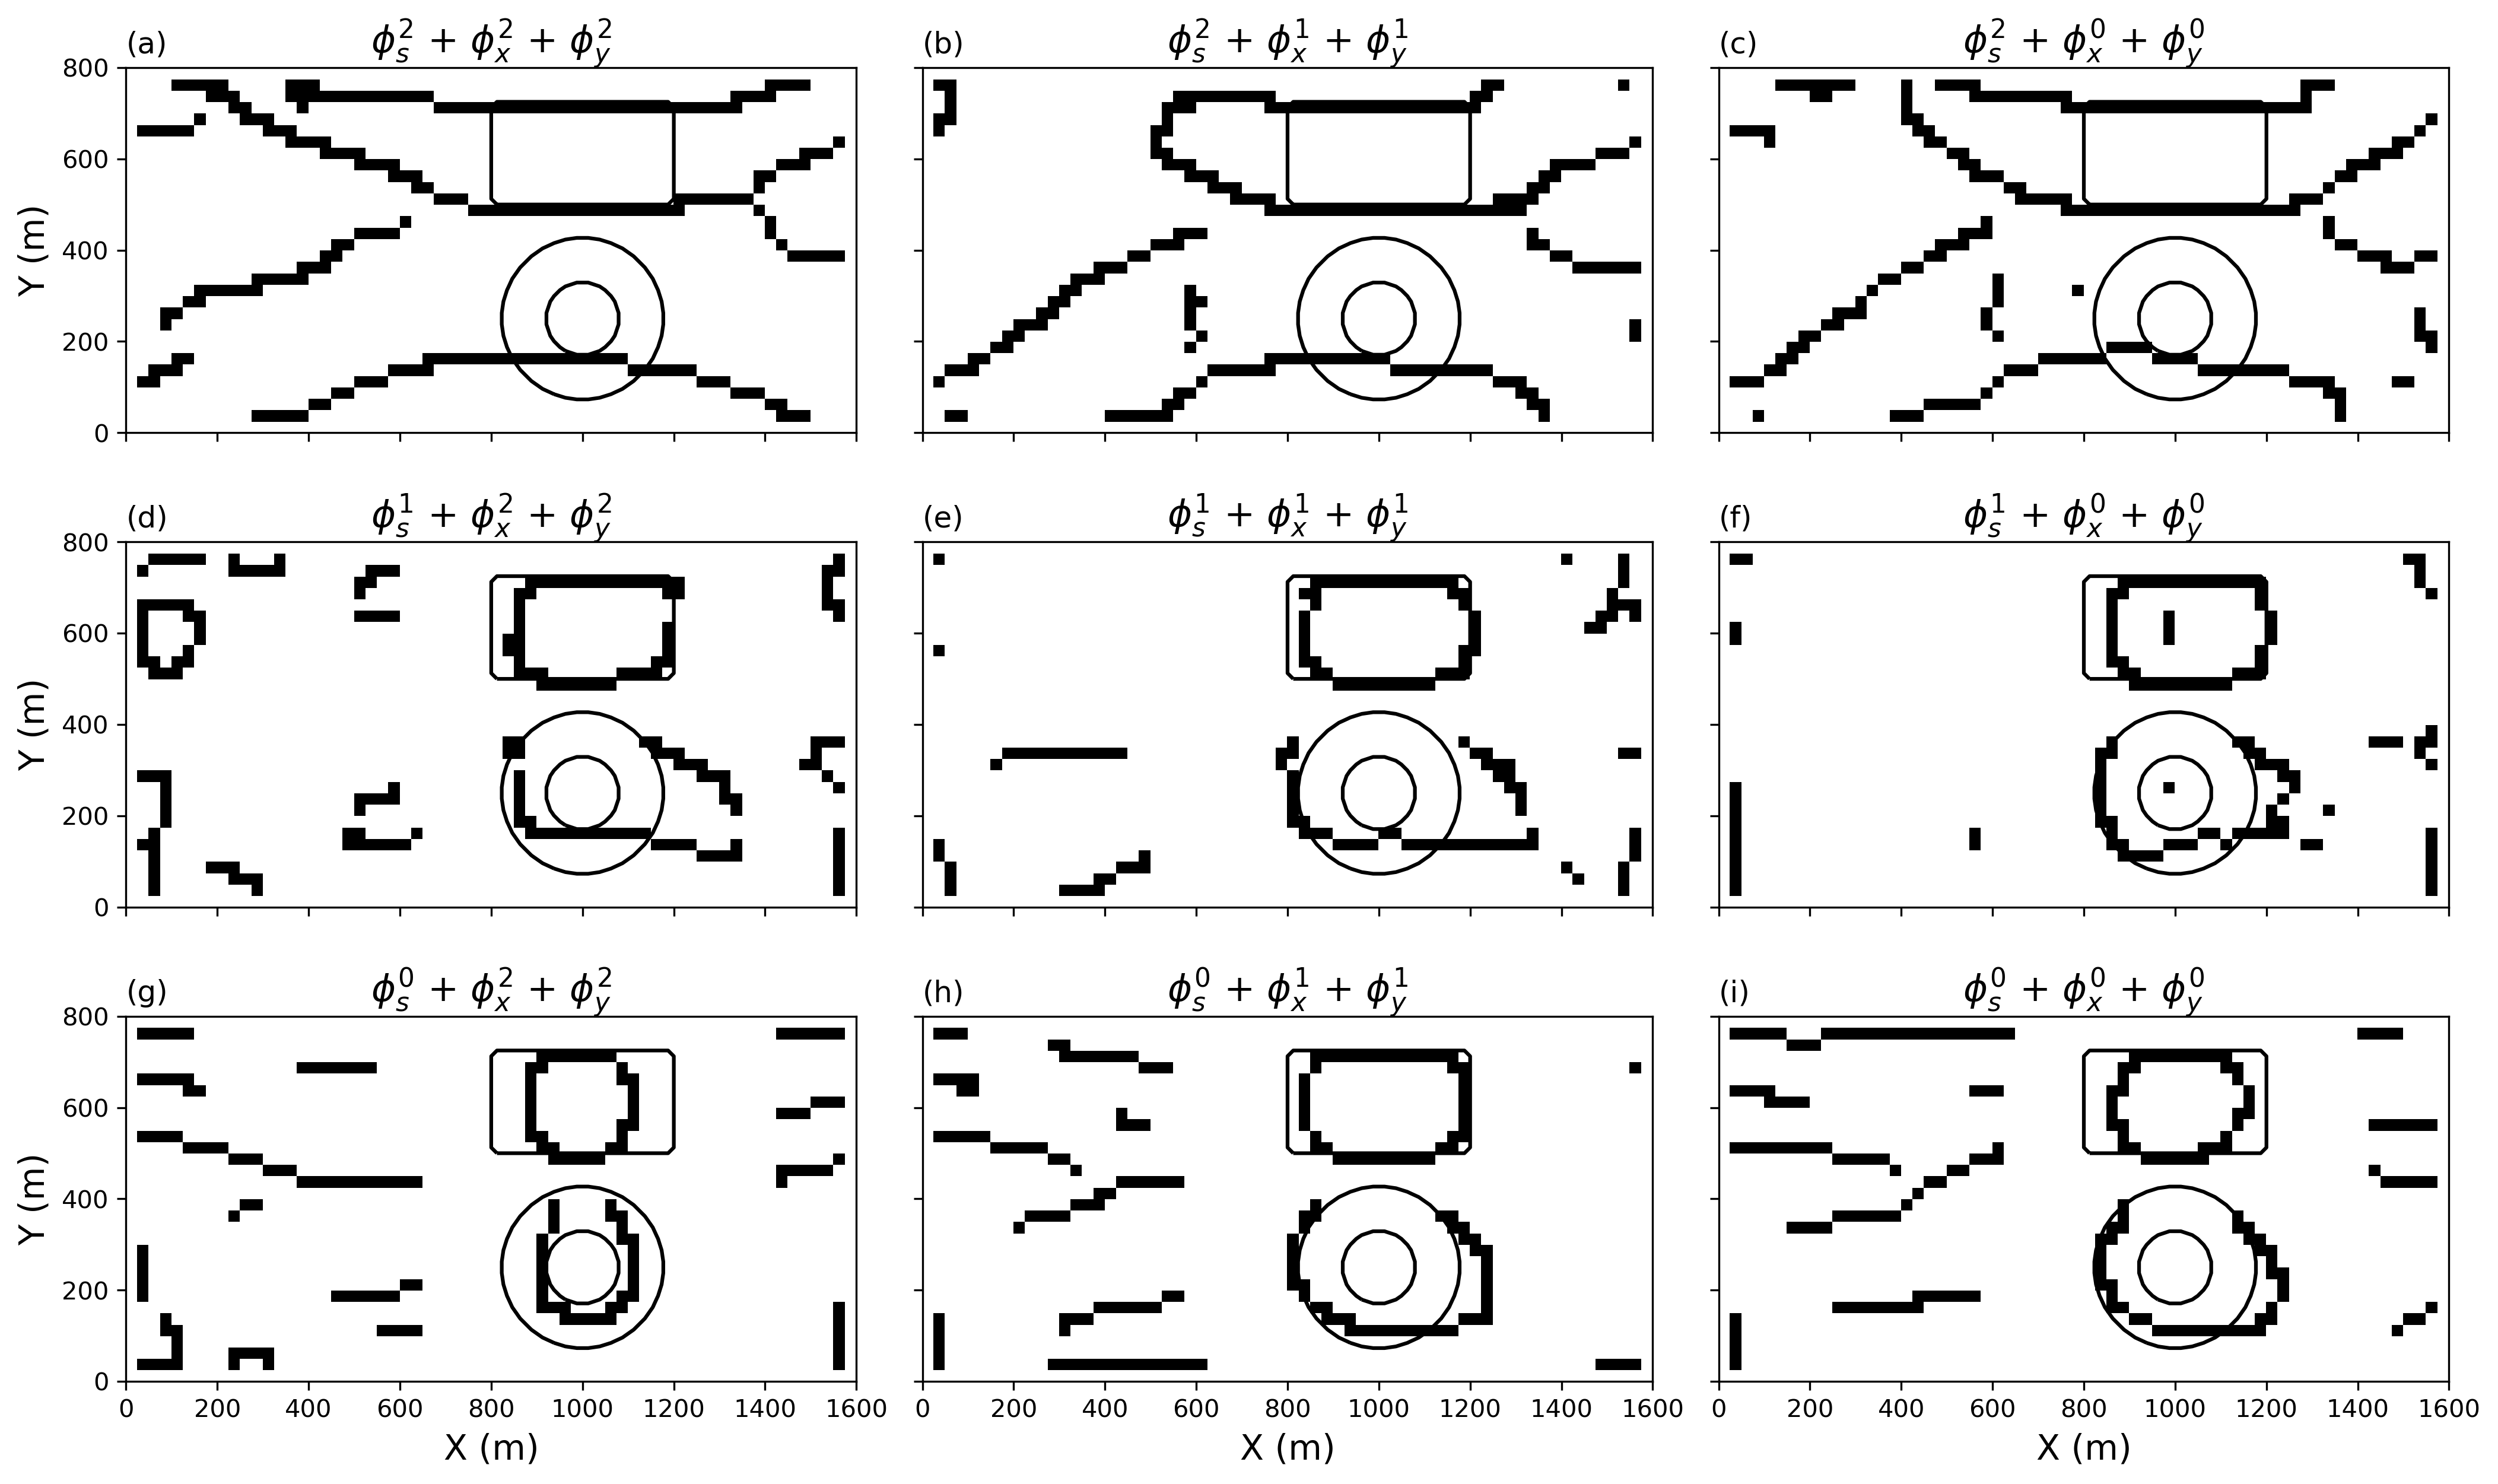
\includegraphics[width=\columnwidth]{Figures/Tomo2D_CannyModels.png}
\caption{Parametric representation of the nine inverted models derived form the Canny edge detection algorithm.}
\label{CannyEdges}
\end{figure}

From this simplified representation of each model, we perform a moving window correlation $r_{\mathbf{m}_i\mathbf{m}_P}$ between the average PCA model $\mathbf{m}_P$ and each of the $\mathbf{m}_i$ solutions:
\begin{equation}
r_{\mathbf{m}_i\mathbf{m}_P} = \frac{\sum_{j=1}^n (m_{ij} - \bar m_{i})({m_{Pj}-\bar m_{P}})}{\sqrt{\sum_{j=1}^n(m_{ij} - \bar m_{i})^2\sum_{j=1}^n(m_{P} - \bar m_{Pj})^2}}
\end{equation}
where $\bar m_{i}$ and $\bar m_{P}$ are the average model and PCA model values inside the window denoted by the subscript $j$.
The parameters $p_s,\: p_x,\: p_y$ associated with the highest correlation are used in a weighted average as defined in \eqref{weightedaverage}. The process is repeated over the entire model space. For our example we use $20 \times 20$ pixels window. The recovered $\mathbf{p}_s$ and $\mathbf{p}_x,\:\mathbf{p}_y$ values are presented in Figure~\ref{MixedNorms}(a) and (b) respectively. We note that the norm on the model gradients is generally larger in the bottom region of the model corresponding to the location of the smooth positive anomaly.
\begin{figure}
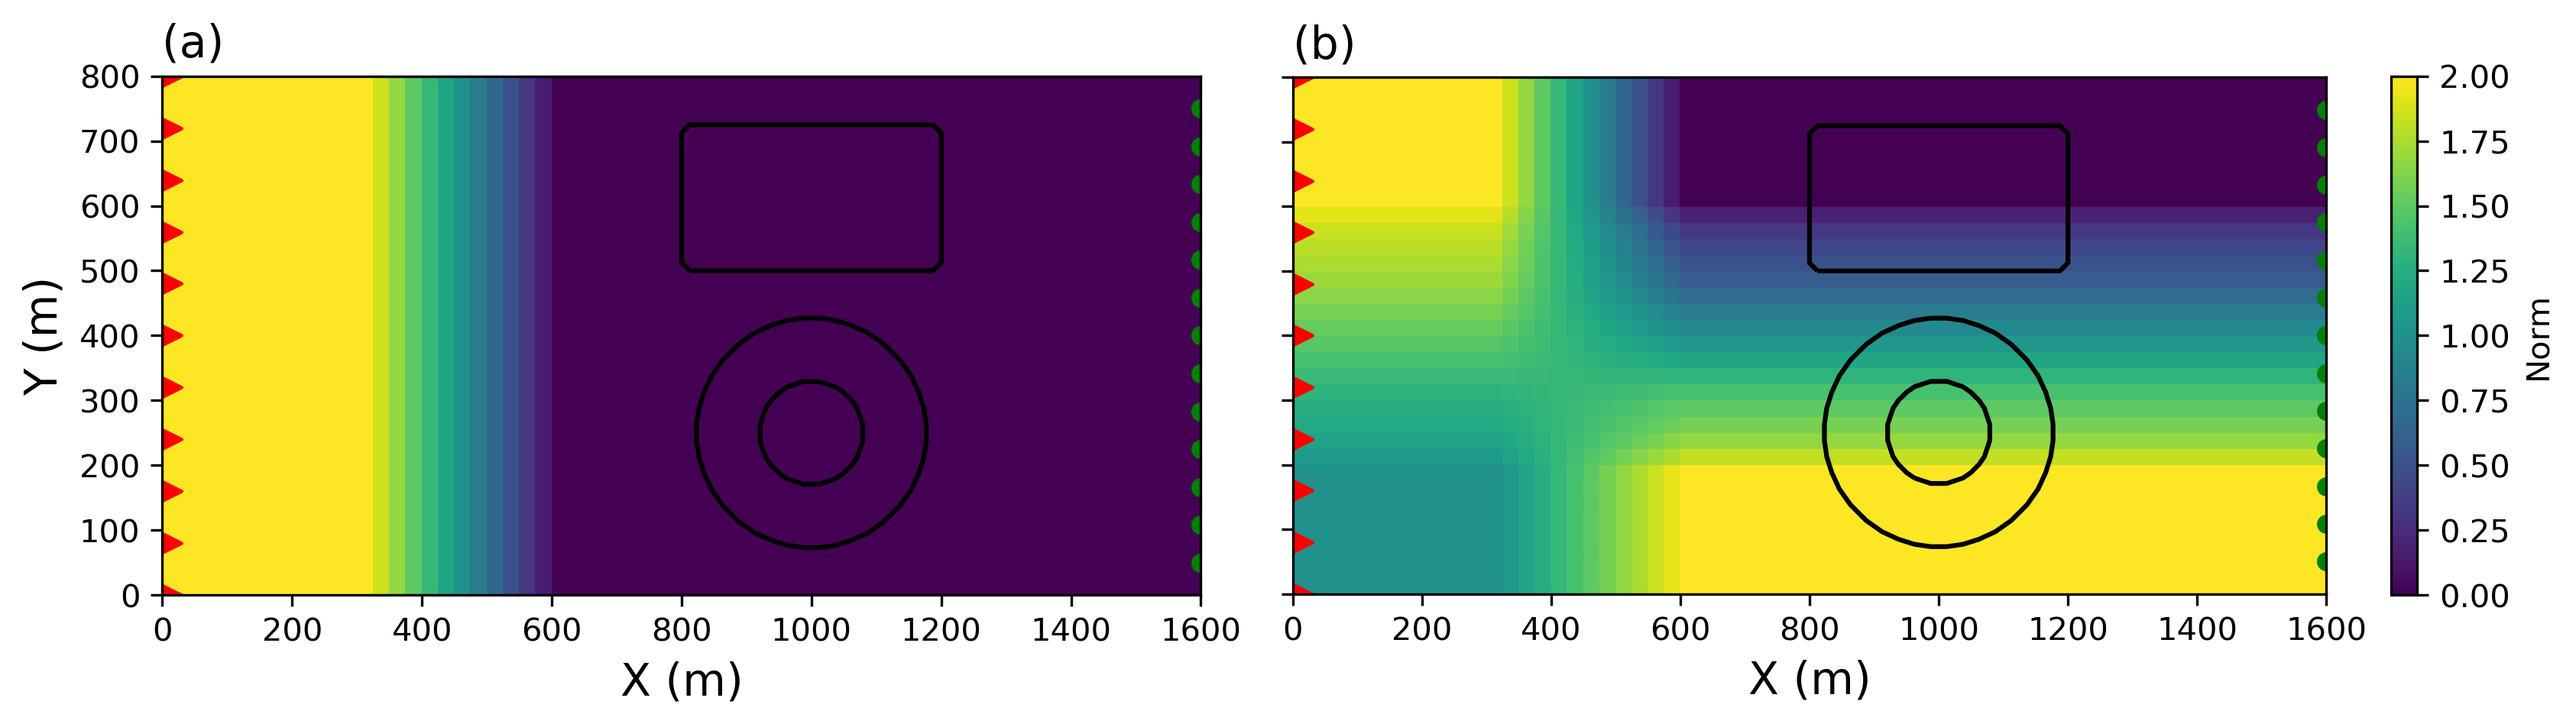
\includegraphics[width=\columnwidth]{Figures/Tomo2D_Average_pq.png}
\caption{Local $p$-values on the (a) the model norm $\phi_s^{p_s}$ and (b) model gradients $\phi_{x}^{\:p_x}$, $\phi_{y}^{\:p_y}$ extracted from the solution space.}
\label{MixedNorms}
\end{figure}

We now define Scaled-IRLS weights on a cell-by-cell basis as:
\begin{equation}\label{mixedIRLS}
\begin{split}
\mathbf{\hat R}_s &= \text{diag} \left[\boldsymbol{\gamma}_s \circ \:{\Big( ({{\mathbf{m}^{(k-1)} - \mathbf{m}^{mref}}})^{2} + \epsilon_s^2 \Big)}^{\circ\:\mathbf{p}_s/2 - 1} \right]^{1/2} \;, \\
\mathbf{\hat R}_x &= \text{diag} \left[\boldsymbol{\gamma}_x \circ\:{\Big( ({{\mathbf{D}_x\;(\mathbf{m}^{(k-1)} - \mathbf{m}^{mref})}})^{2} + \epsilon_x^2 \Big)}^{\circ\:\mathbf{p}_x/2 - 1} \right]^{1/2} \;,\\
\mathbf{\hat R}_y &= \text{diag} \left[\boldsymbol{\gamma}_y \circ\:{\Big( ({{\mathbf{D}_y\;(\mathbf{m}^{(k-1)} - \mathbf{m}^{mref})}})^{2} + \epsilon_y^2 \Big)}^{\circ\:\mathbf{p}_y/2 - 1} \right]^{1/2} \;,\\
\end{split}
\end{equation}
where $\circ\mathbf{p}_s$, $\circ\mathbf{p}_{x}$ and $\circ\mathbf{p}_y$ define the element-wise Hadamard power and $\boldsymbol{\gamma}_s \circ$, $\boldsymbol{\gamma}_x \circ$ and $\boldsymbol{\gamma}_y\circ$ are the element-wise scaling multiplications defined in \eqref{etaScale}. In this fashion, the approximated mixed norm regularization can vary on a cell-by-cell basis.

Finally we proceed with our SVMN inversion. The data are now inverted using the extracted local parameters, applied on a cell by cell basis, and the result is shown in Figure~\ref{FinalMixedNorm}. There is good correspondence with the true model: both the low velocity blocky anomaly and the high velocity smooth anomaly are imaged at the right location, with the right shape and near their respective seismic velocity. It is worth noting that we have achieved this result without direct input from the user, other than choosing a window size at the parameter extraction phase.
\begin{figure}
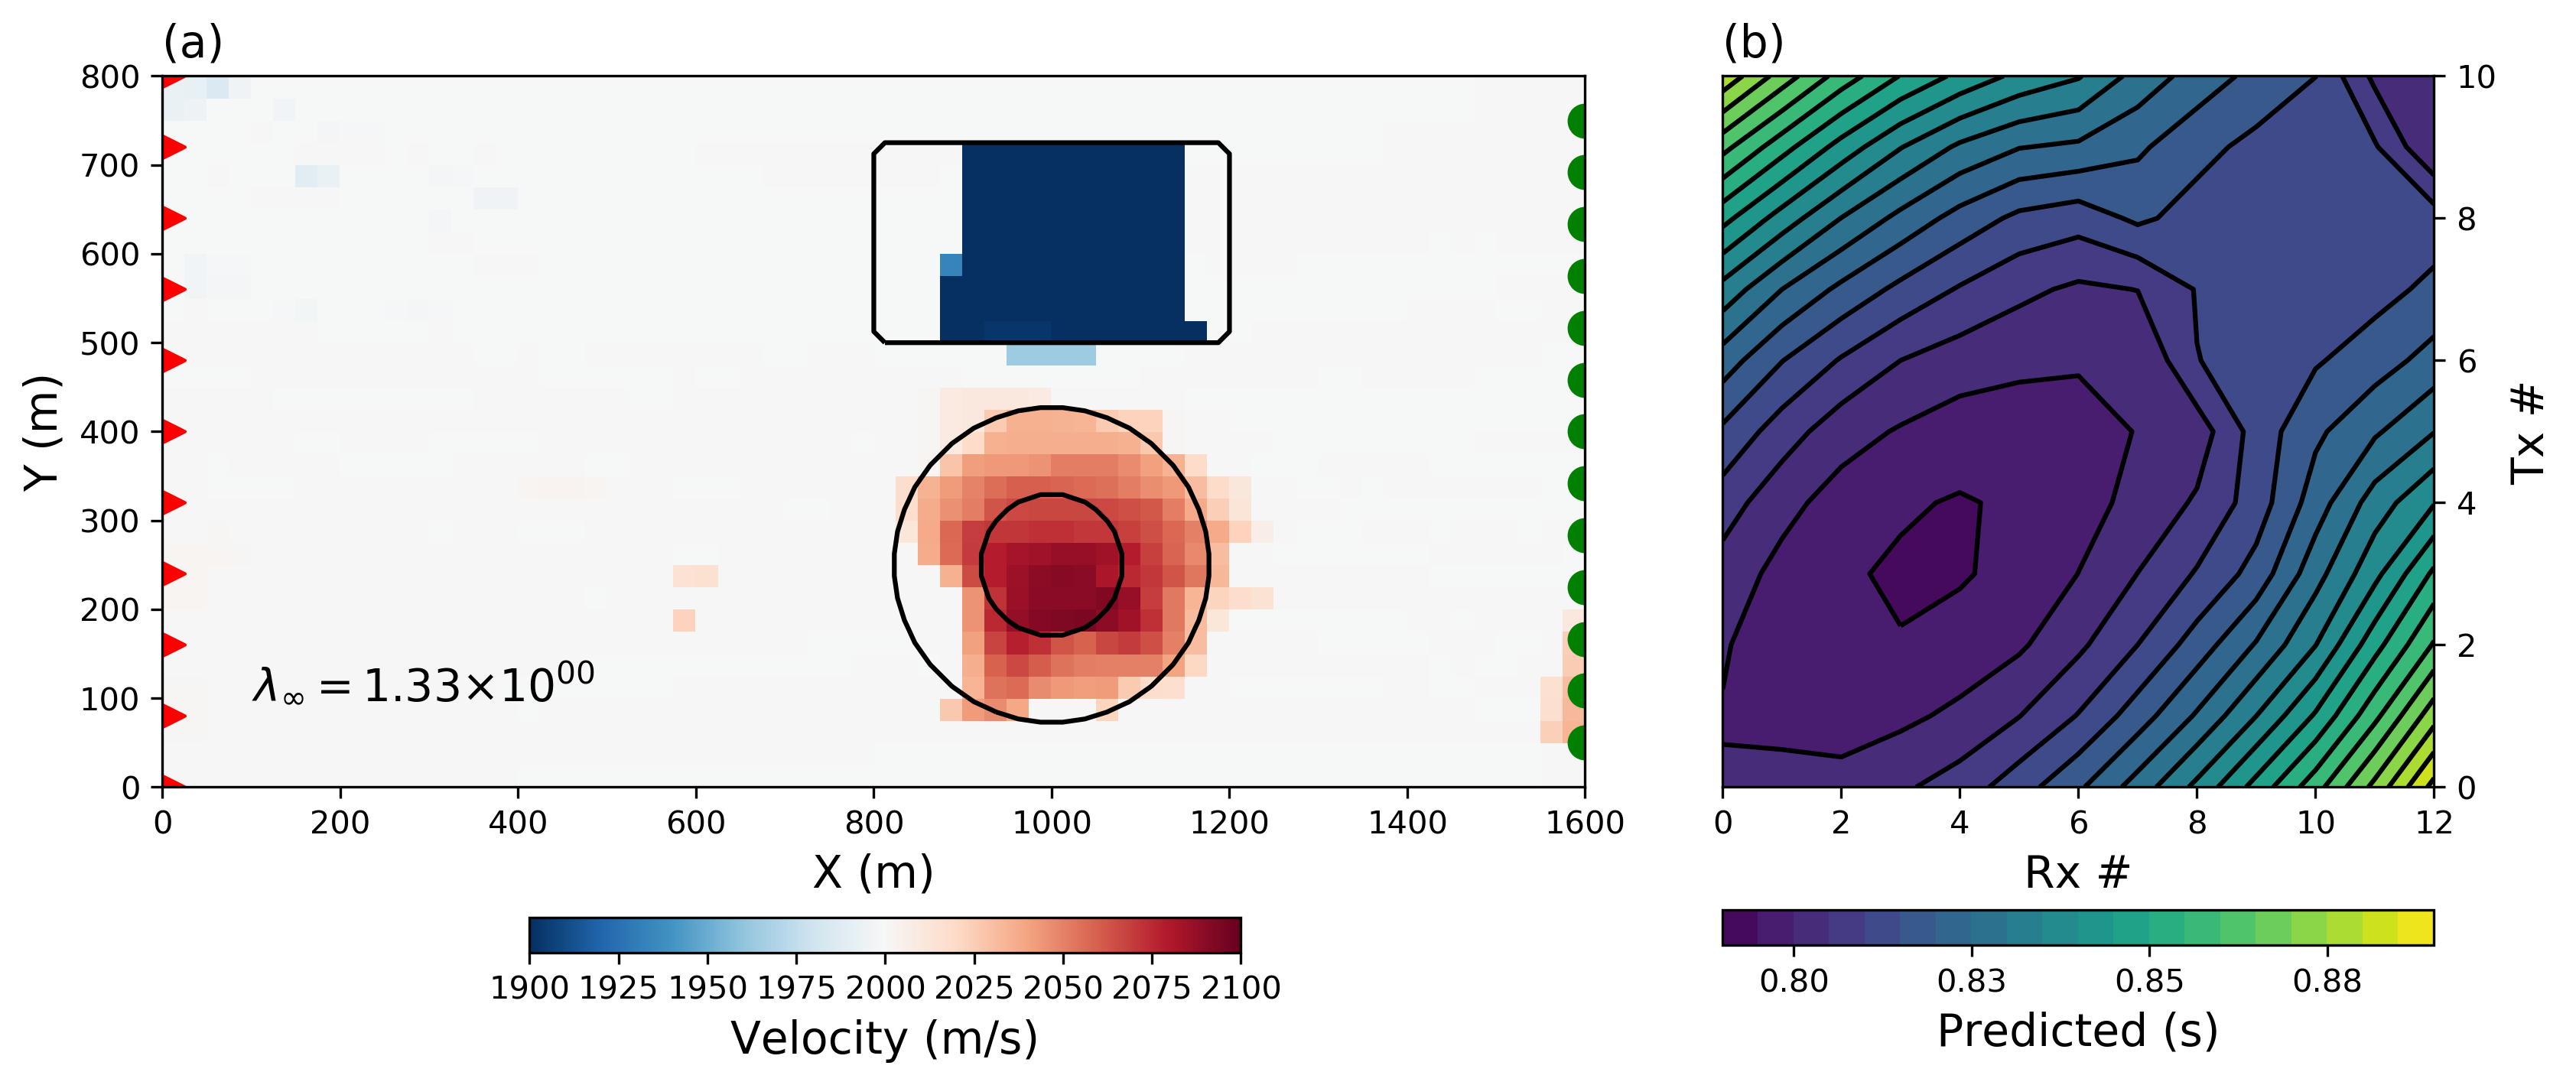
\includegraphics[width=\columnwidth]{Figures/Tomo2D_Reinverted_Variance.png}
\caption{(a) The final SVMN inversion result (b) predicted data. Contour lines are shown in (a) for the true position and shape of the velocity anomalies.}
\label{FinalMixedNorm}
\end{figure}



\section{Case study: DO-18/27 airborne magnetics}

We now use our algorithm to invert airborne magnetic survey acquired over the DO-18/27 diamondiferous kimberlite pipes previously shown in Figure~\ref{TKC_Data}.
The deposit is located 30 km SE from the Lac de Gras region, Northwest Territories. The DO-18/27 kimberlites pipes are more conductive and susceptible than the host archean rocks and easily identifiable from airborne surveys \cite[]{Pell1997, Devriese2017a, Fournier2017}. They are also associated with a large network of magnetic dyke swarms. Our goal is to better recover the shape of compact kimberlite pipes as well as the narrow and elongated dykes.

At the time of acquisition, the inducing field strength, inclination and declination were 59,500 nT, $83^\circ$ and $19.5^\circ$ respectively.
As a first step, we rotate the magnetic data $30^\circ$ clockwise in order to align the strike of dykes along the Cartesian directions (not shown here). We assign $5$ nT uncertainty on the data. We discretize the Earth into 25 m cubic cells and invert the data with the conventional smooth $\ell_2$-norm assumption with the open-source \texttt{SimPEG} package \cite[]{Cockett2015}. As shown in  Figure~\ref{TKC_Results}(a), the magnetic dykes appear to break between each survey line due to large flight line separation. Considering the regional geology, the magnetic dykes are likely to be continuous throughout the region and they should be better represented by plate-like bodies.

As previously done on the synthetic 2D model, we proceed with a series of inversions to sample solution space. Since we are now dealing with a 3D problem, a large number of combinations of norms for $p_{s,x,y,z}=2,1,0$ is possible. We are mostly interested in accentuating trends along the dykes and better resolving the shape of the kimberlite pipes. Lowering the norm applied to specific model gradients promotes the recovery of piecewise continuous bodies along the same direction. So rather than applying an $\ell_p$-norm on all model gradients equally, we want to reduce the $p$-value on each gradient independently. This would, in theory, require 81 inversions if we set $p_{s,x,y,z}=2,1,0$.
We narrow down our analysis to eight models based on the following criteria.
(a) We expect the geology to extend vertically, but the weak depth resolution of magnetic data does not allow to distinguish clear trends for steeply dipping bodies. So we restrict our analysis to smooth vertical models ($p_z=2$).
(b) We want to concentrate on continuity and character of the dykes in the two orthogonal directions. We therefore vary $p_{x,y}=2,1,0$. Figure~\ref{TKC_Results}(b)-(i) presents horizontal sections at 75 m below the surface for eight subsequent inversion trials.
We note that sparsity imposed on the model gradients along a specific Cartesian direction helps in recovering continuous features.
While it is possible to manually divide the survey area into regions with variable norms \cite[]{FournierDavis2016a}, we will attempt to extract these preferential orientations through the methodology prescribed in the previous section.
\begin{figure}
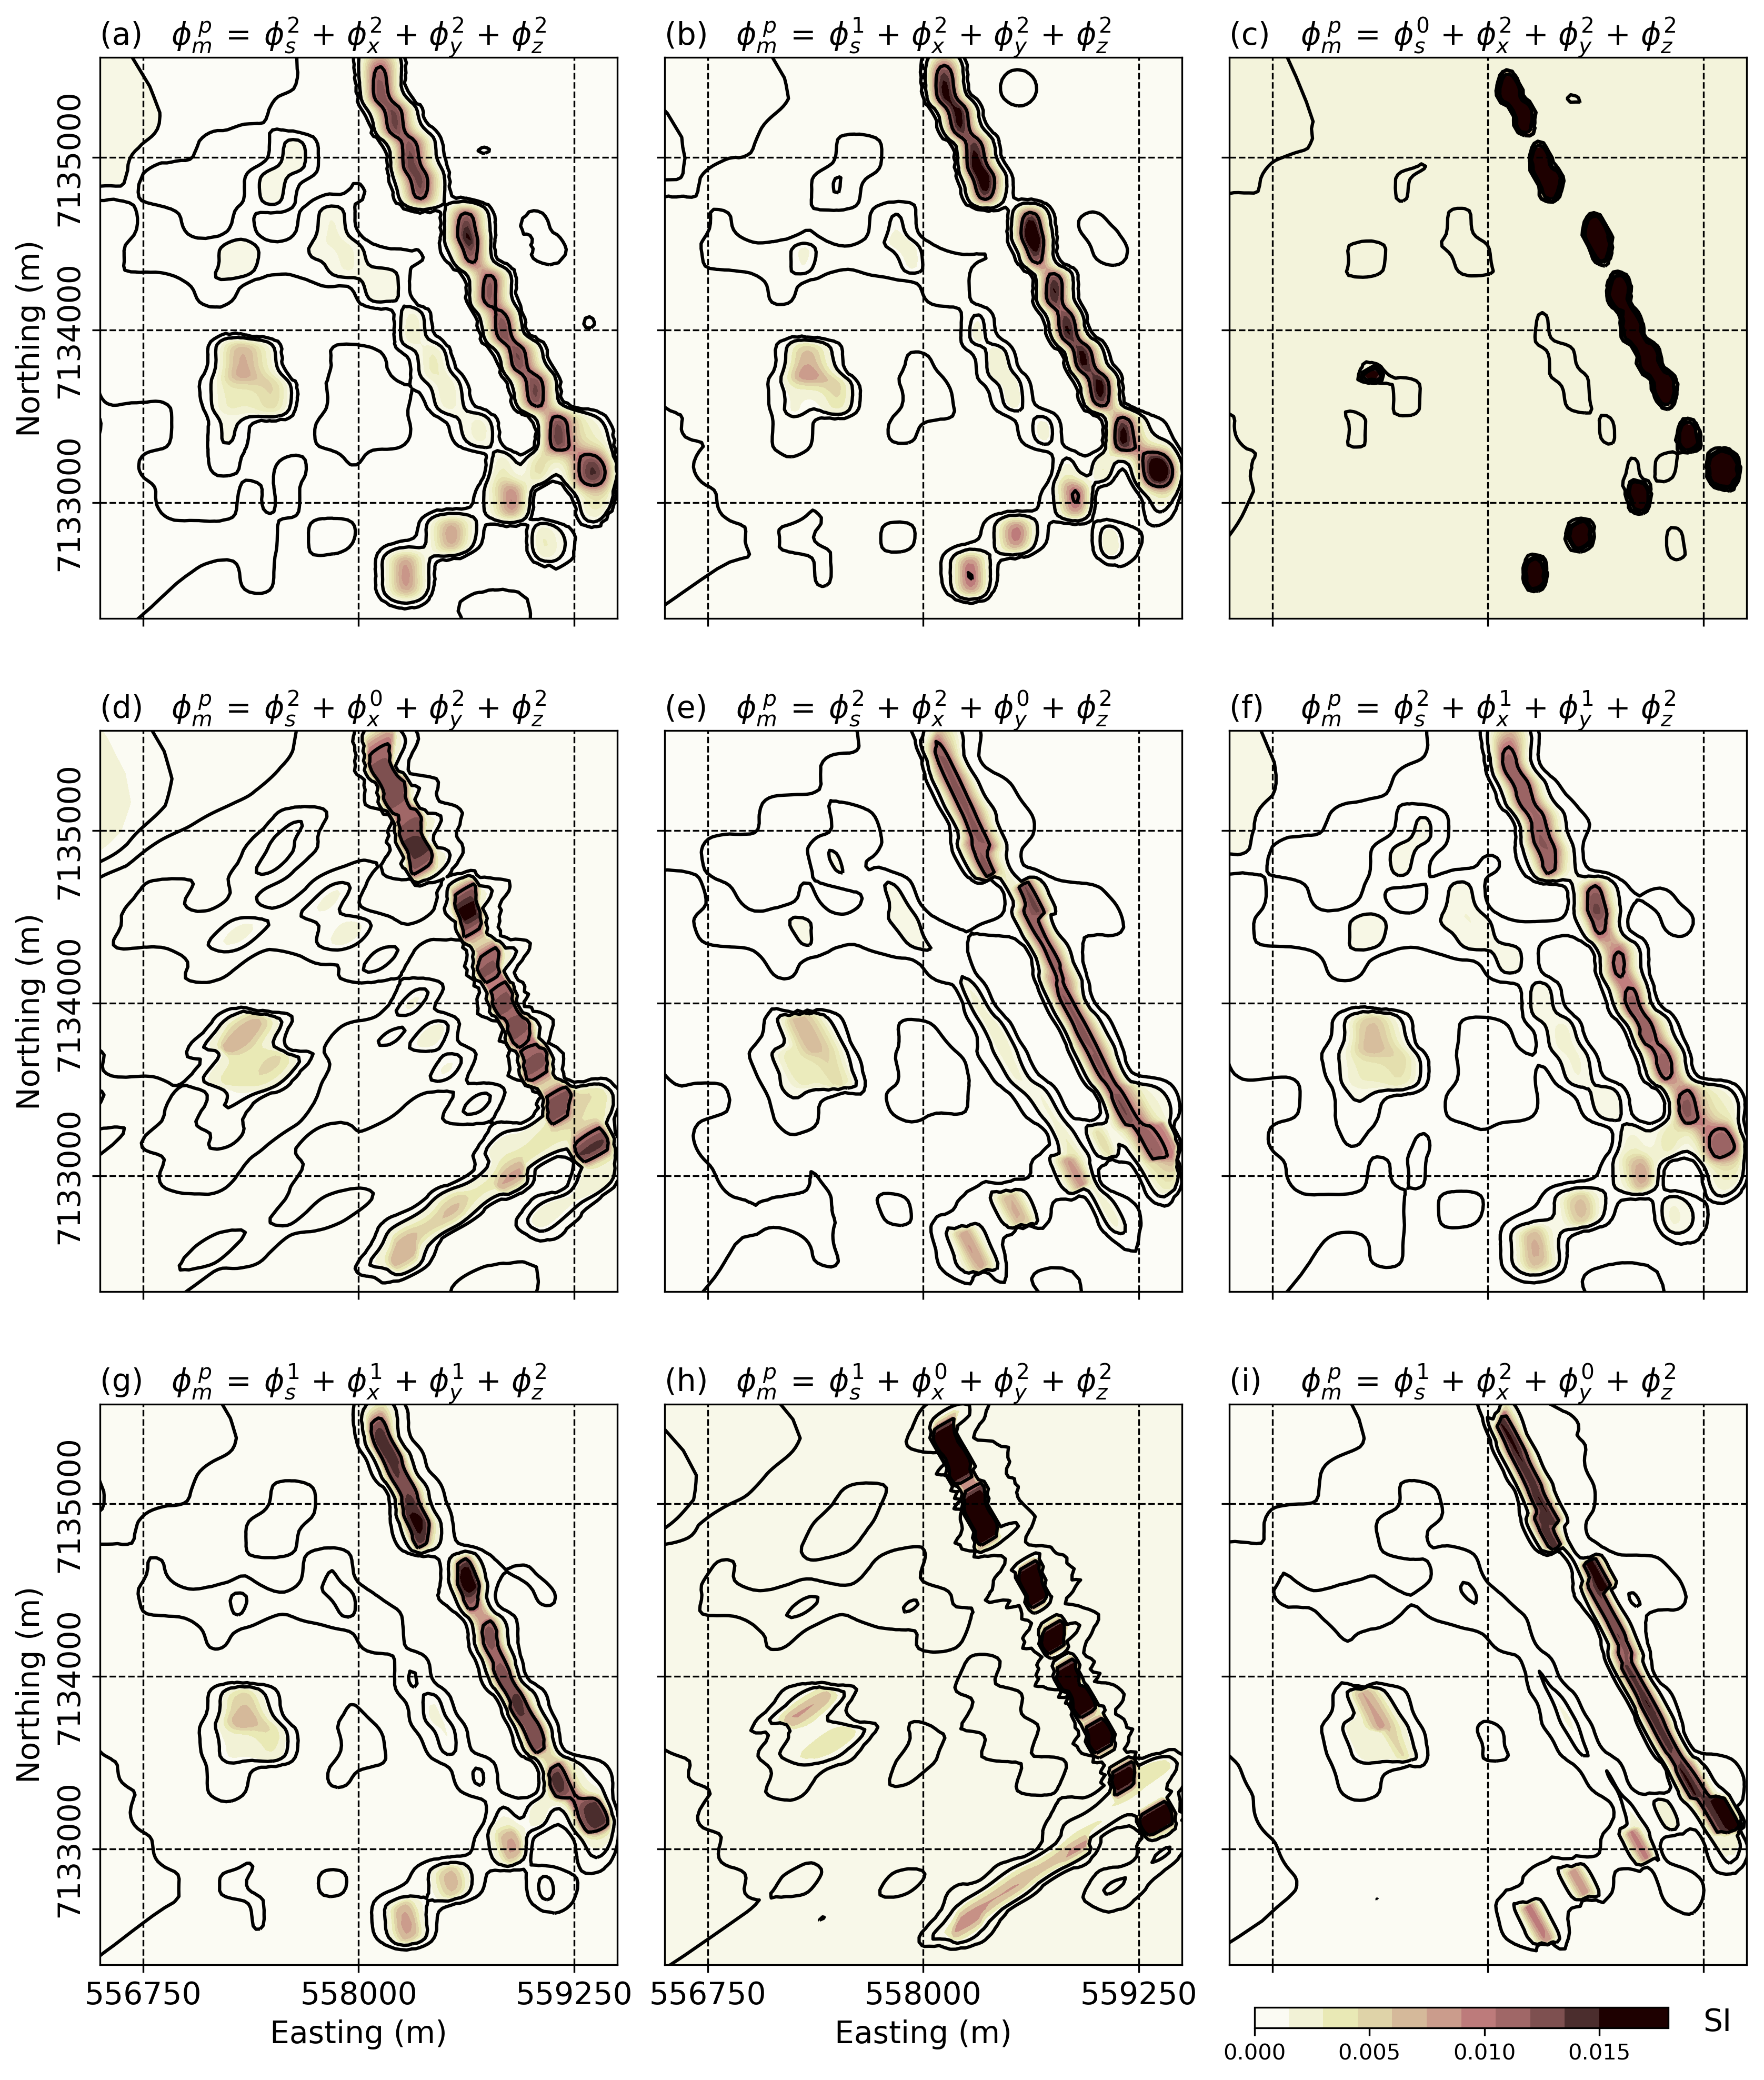
\includegraphics[width=\columnwidth]{Figures/Results_MAG_TKC_Results_All.png}
\caption{Horizontal sections through nine inversions of the airborne magnetic data over TKC after rotating back to UTM coordinates. Sparsity parameters are imposed along different directions to enforce lateral continuity.}
\label{TKC_Results}
\end{figure}

The following analysis steps are performed in 2D along the same horizontal section at 75 m depth.
We restrict our analysis to this horizontal depth section for three reasons: (1) we want to sample the cross-section of the DO-27 kimberlite pipe buried under a thick layer of glacial till, (2) near surface features recovered in most models are dominated by the flight line separation, which we are trying to suppress with this process, (3) we have stronger confidence in the geometry of the geology in 2D.

We first perform a model averaging through a PCA followed by an edge detection analysis. The selection of an optimal window size and detection parameters used by the Canny algorithm is problem specific as it depends on the size and shape of features of interest. We used a $10\times 10$ cells moving window ($250\times250$ m). Figure~\ref{TKC_Params}(a) presents the recovered $\mathbf{m}_P$ overlaid by the edge solution. The different dyke orientations are clearly visible, as well as the circular anomalies associated with the kimberlites pipes. We then proceed with a parameter extraction step based on the correlation between $\mathbf{m}_P$ and the solution space. Sparse norms for the model and its gradients are shown in Figure~\ref{TKC_Params}(b) to (d)
\begin{figure}
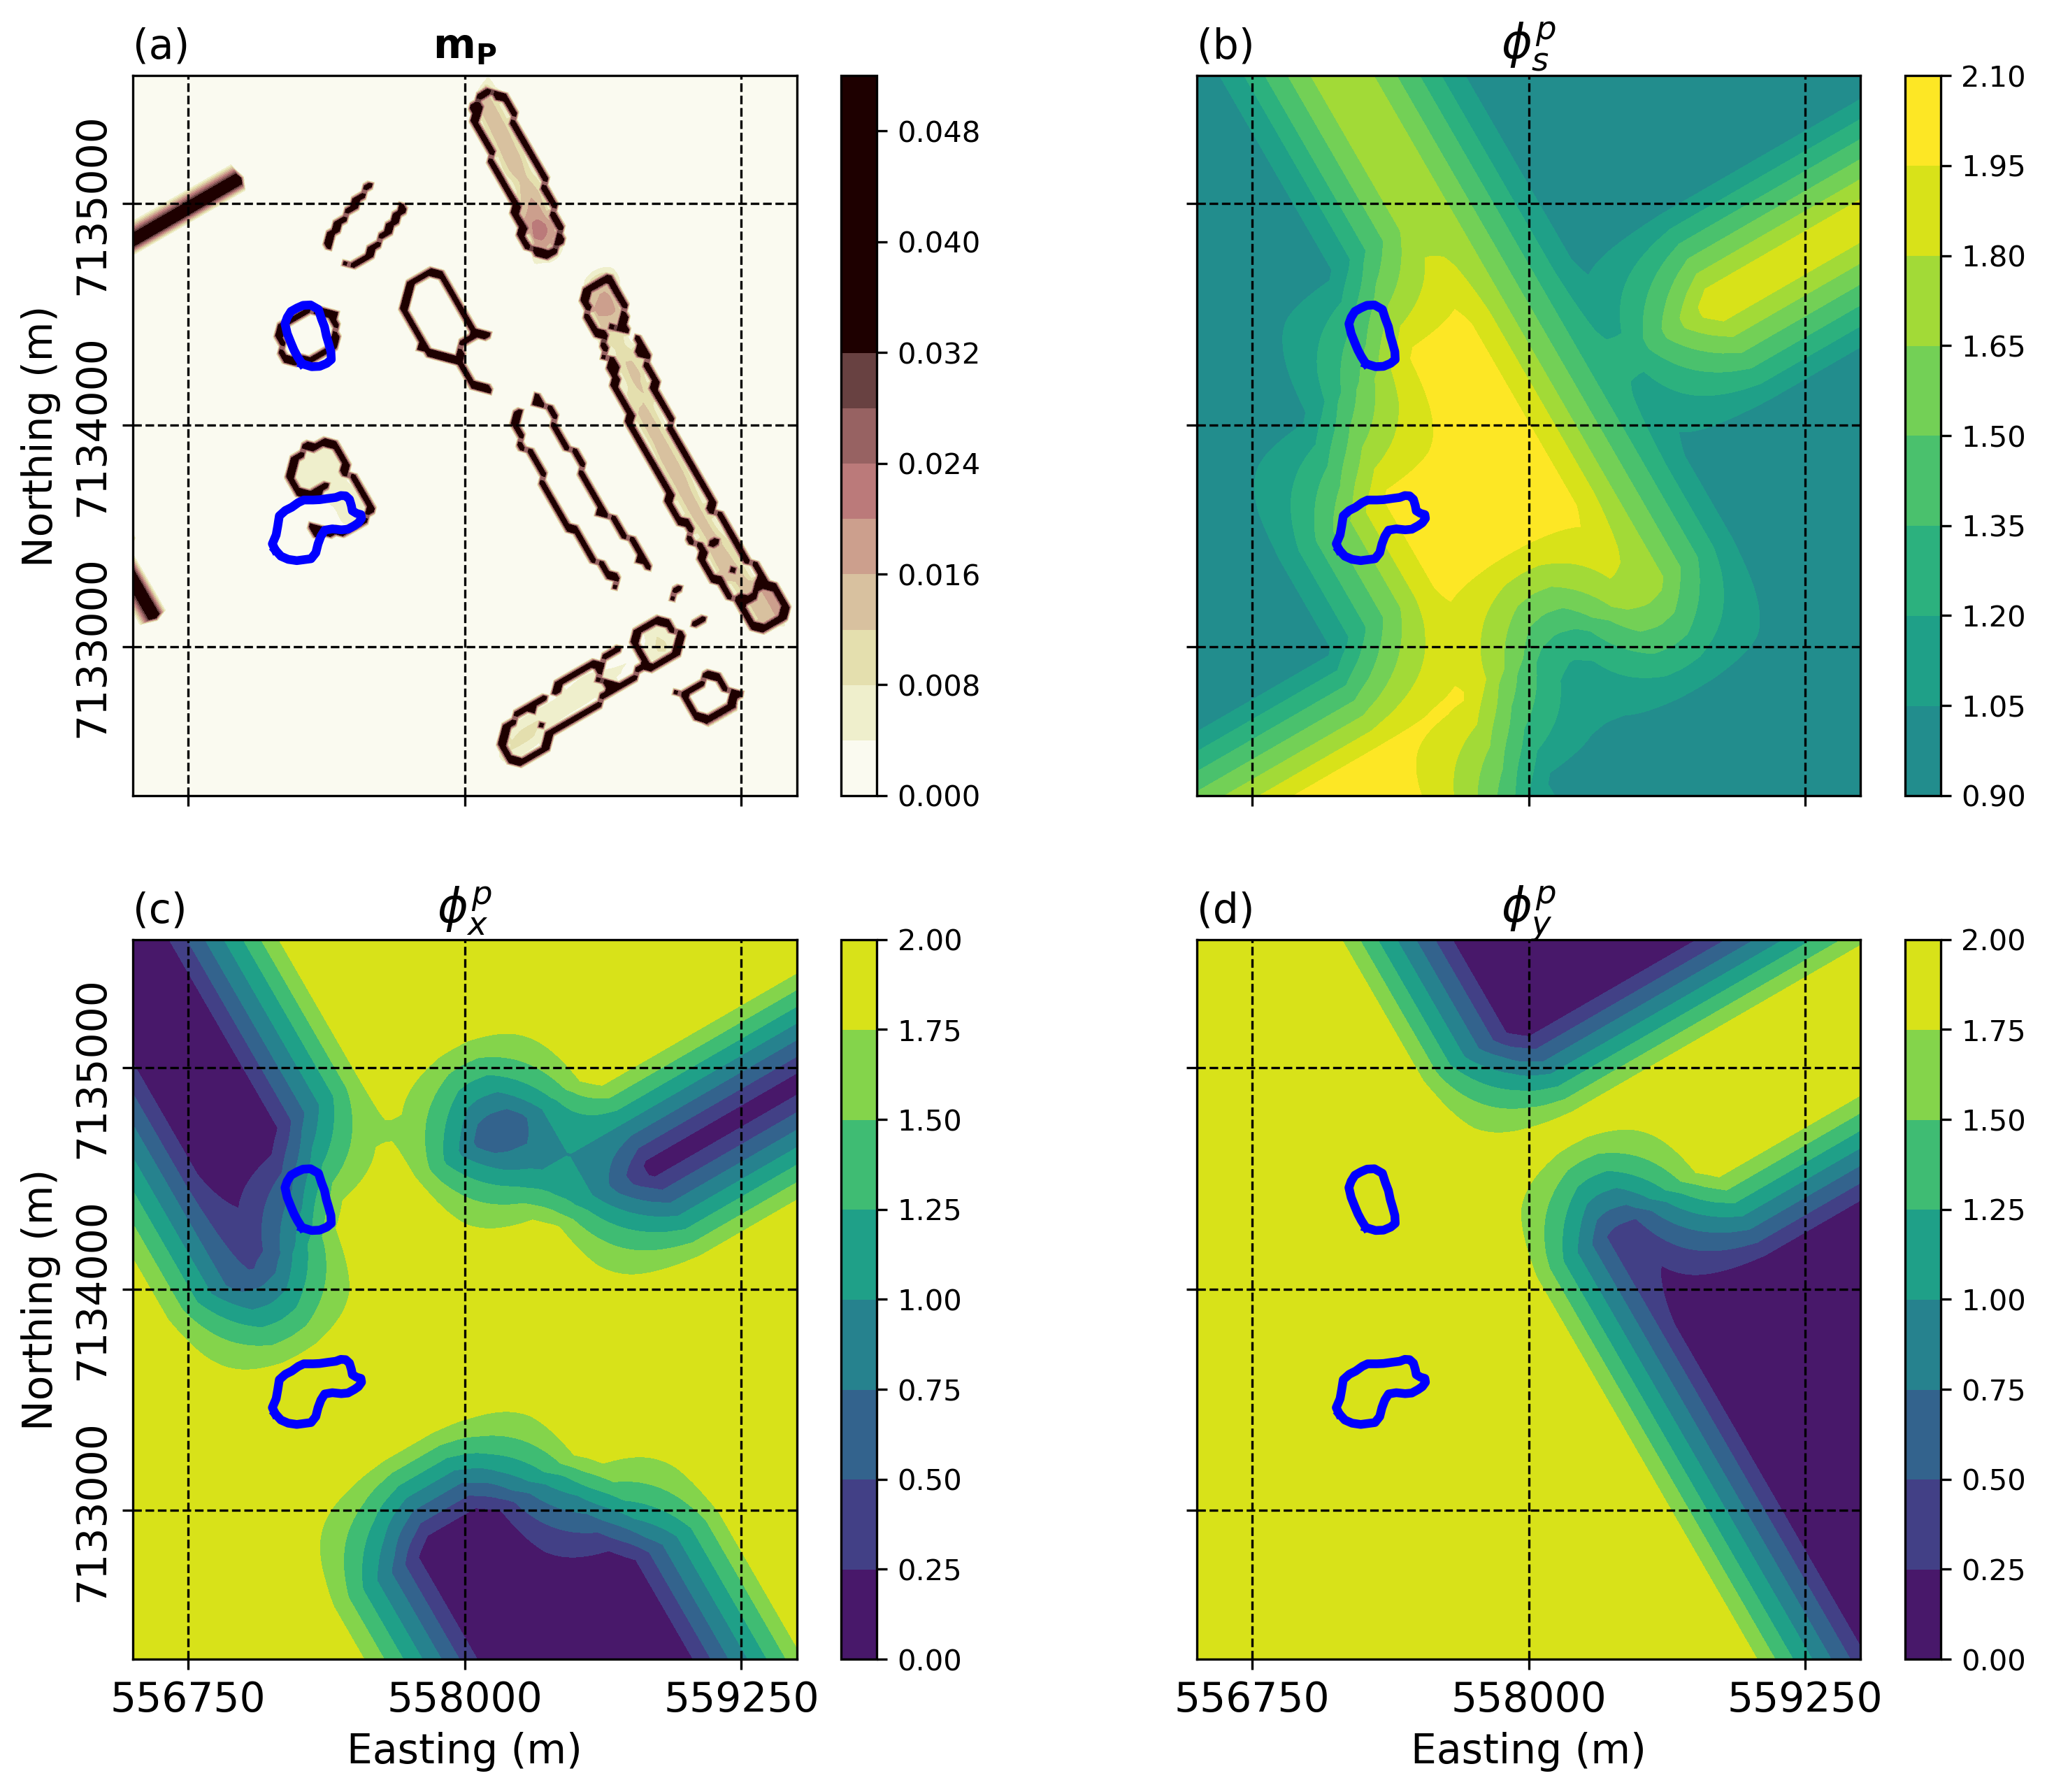
\includegraphics[width=\columnwidth]{Figures/MAG_TKC_LocalParam.png}
\caption{Estimated parameters from the correlation between all the inverted models. (a) the averaged PCA model $\mathbf{\bar m}_P$ and its Canny edge representation. (b-d) Average $p$-values for $\phi_s^{\:p}$, $\phi_x^{\:p}$ and $\phi_y^{\:p}$ respectively. The outlines of the kimberlite pipes are shown for reference.}
\label{TKC_Params}
\end{figure}

In a final step, we proceed with the SVMN inversion. This yields the model presented in Figure~\ref{TKC_Final}. The solution highlights the important features in the region:
\begin{enumerate}
\item Two continuous and narrow anomalies striking at $315^\circ$N. Both dykes show the same apparent break, which may correspond to left-lateral faulting event at Northing 71346500.
\item A third dyke striking at $60^\circ$N, appears to overprint the signature of the weakest dykes
\item The magnetic anomaly associated with DO-18 in the north coincides with the location of the known pipe.
\item The southern anomaly related to DO-27, shows higher susceptibility along the northern edge of the pipe. This anomaly was the initial target identified by the exploration team and later drilled. It is now understood that the main magnetic signal originating from DO-27 is associated with the hypabyssal kimberlite (HK) unit, a sheet-like intrusive mafic unit that has low diamondiferous content. Our inversion is thus consistent with the geology.
\end{enumerate}
\begin{figure}
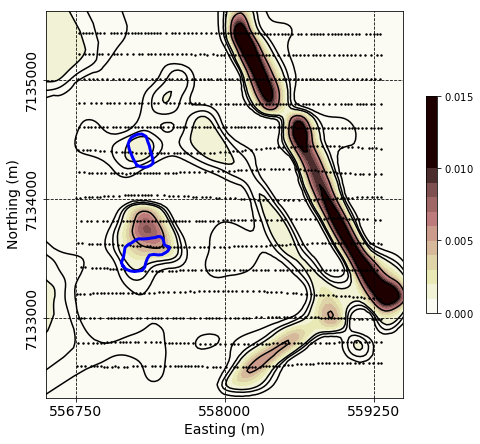
\includegraphics[width=\columnwidth]{Figures/MAG_TKC_FinalModel.png}
\caption{Final mixed-norm susceptibility model recovered over the DO-18/27 kimberlite pipes shown with blue outlines.}
\label{TKC_Final}
\end{figure}
This final solution is an improvement over all nine previous inversions as it has managed to recover both elongate and continuous dykes striking in different directions, as well as compact isolated kimberlite pipes. A similar result has previously been shown in \citet{Fournier2015}, but that required tedious manual effort to select the norm models. We have accomplished the same result by using only the geophysical data and an entirely automated process for selecting parameters.


\section{Conclusion}
The geophysical inverse problem is inherently non-unique and the character of the solution is controlled by a regularization function that consists of multiple terms each of which is designed to affect the final outcome in a specific way. \emph{Smallness} penalties force the solution to be close to a reference model; \emph{roughness} penalties are focused on spatial variation. When composited into a final regularization, each term is pre-multiplied by a constant ($\alpha$ in our notation). Selecting appropriate values of $\alpha$ is challenging because the numerical value of the penalty depends upon the selected $p$-norm as well as the numerical discretization used to evaluate derivatives. As the number of penalty terms grows, and especially when each involves a different $p$-norm, pre-specifying the $\alpha$ values becomes challenging, time consuming and sometimes ineffective. In addition, solving an $\ell_p$-norm problem when $p<1$ poses additional challenges because the problem is no longer convex. To address these challenges we take the following approach: (i) we replace the $\ell_p$ norms with the Lawson norm and, at each iteration, solve a local linear problem using IRLS; (ii) we use a two-stage process where, in the first stage, all penalties are $\ell_2$ and in the second stage they are replaced by their final $\ell_p$ values; (iii) we replace the spatial derivatives with finite differences. This makes all penalty terms dimensionally equivalent and allows the $\alpha$ parameters to have a default value of unity; (iv) we rescale the gradients at each IRLS iteration so that all penalty terms can be equally influential in the final solution; (v) we introduce a proportionality ratio of the gradient vectors, ${\lambda_\infty}$, to measure success in achieving equal contribution from different terms in the regularization; (vi) we cool the parameter $\epsilon$ in the Lawson norm and use ${\lambda_\infty}$ to indicate whether a slower cooling is needed. Although we have portrayed our algorithm as one that produces a solution in which all terms in the regularization are equally effective in the final inversion, it is trivial to incorporate different weightings; ${\lambda_\infty}$ then reflects the desired relative weightings.

Our inversion algorithm allows us explore two important items. The first is to sample the solution space associated with $\ell_p$-norms. The character of the model changes markedly with $p$-value and inversions with different combinations of norms provides insight about which features might be required by the data and their geologic character. The importance of seeing multiple solutions to the same inverse problem cannot be overestimated.

The second important item is to construct a solution that encompasses different types of geologic features with a single domain. The geology at Tli Kwi Cho is a motivating example. At this level of complexity however, there are too many $p$ parameters for a user to specify manually and some way to automate the procedure is required. We provide one strategy: (i) carry out a suite of $\ell_p$ inversions and build an ensemble of models; (ii) extract common features using a PCA analysis and build an average model $\mathbf{m}_P$; (iii) in a windowed environment, perform correlations of ensemble member with $\mathbf{m}_P$; for computing correlations we map the models to their Canny Edge representation; (iv) the suite of $p$-values corresponding to the largest correlation coefficient is assigned to the cell at the center of the moving window; (v) a final inversion, in which each cell has its own suite of $p$-values, is carried out. This should be a candidate for a best model to interpret geologically.

Implementing the above process using SVMN has provided us with an image of magnetic susceptibility at TKC that is better related to geology than any other single inversion we have done. The methodology by which we generate and select the ensemble of possible solutions and the analysis by which we extract the SVMN parameters deserves further investigation. Finally, from a geometric perspective, we have so far used penalty terms on the model gradients measured along the three Cartesian directions. This is only appropriate if geological features are intersecting at right angles. Future work could increase the flexibility of the inversion by allowing gradient measures at variable angles.



\section{Acknowledgment}
The Authors would like to thank Peregrine Diamond Ltd. for giving us access to the airborne magnetic data. Special thanks goes to the \texttt{Scikit Learn} and \texttt{SimPEG} development teams for their contribution to the open-source community.
\bibliographystyle{gji}
\bibliography{reference}


\end{document}
